\documentclass[11pt,letterpaper]{article}
\input{headings}
\newcommand \recipeName {Chicken Filling}
\newcommand \fileName {ChickenFilling}
\chead{\recipeName}

\begin{document}
\input{title}

This is a general-purpouse chicken filling that can be used for many recipes including Pastel\~ao, risolis, past\'eis. It is also delicious in a simple pressed sandwich or as a topping for pizza. I got this recipe from my mother and I know that she uses it frequently. 
 
\begin{description}

\item[Ingredients:]\ \\
	\begin{itemize}
	\item 1 chicken
	\item 2 clove of garlic
	\item 1/2 Tablespoon of salt
	\item 1/4 tablespoon of freshly grounded black pepper
        \item 2 Tablespoon of flavourless cooking oil (such as canola or sunflower)
        \item 2 cup of water
        \item 1 medium onion
        \item 1 teaspoon of honey
	\item 1 16 oz can of Italian tomatoes
	\item 1 Tablespoon of corn starch
	\item 3 perfect hard-boiled eggs (see \href{HardBoiledEggs.html}{Julia Child's Master Recipe})
        \item Italian parsley
	\end{itemize}

\item[Procedure:]\ \\
	\begin{enumerate}
	\item{\bf Season the Chicken}
	\begin{itemize}
        \item Cut up the chicken (alternatively use chicken breasts only).
        \item Sprinkle chicken with salt.
        \item Place the chicken in a closed container and put it in
              the refrigerator for at least to 1 hour (up to 12 hours).
        \end{itemize}
        \item{\bf Brown the Chicken}
        \begin{itemize}
        \item Heat up the cooking oil on a heavy-bottom sautee pan in moderately high heat.
        \item Lightly brown the chicken on all sides.
        \item Peel and split garlic cloves in half and add to the pot.
        \item Add 1 cup of water, bring to a boil, reduce
          the heat and simmer until the chicken is tender (remove the breast earlier so that they don't dry).
        \item After removing the breasts, keep cooking until all the water have evaporated. Only the fat and brown bits should be in the pan.
        \item Remove the remainder pieces of chicken to a platter to cool off.
        \end{itemize}
        \item{\bf Make the Tomato Sauce}
        \begin{itemize}
        \item Drain all the fat to a small container and reserve.
        \item Add 1 cup of water to the solids in the pan, scrape and let it simmer until you have a rich broth in the pan scraping all the broth from the pan with a rubber spatula.
        \item Pour broth into a small container and reserve.
        \item Dice the onion in very small dice.
        \item Add 2 Tablespoon of the reserved fat to the pan and heat up in moderately high heat.
        \item Add the diced onion and sautee for 5 minutes until the onion start wilting.
        \item Add 1 teaspoon of honey to the onion and continue salteeing until golden brown.
        \item Add the can of tomatoes and the reserved chicken broth.
        \item Let simmer until most of the water has evaporated and the fat is separating from the tomato sauce.
        \end{itemize}
        \item{\bf Debone and dice the chicken}
        \begin{itemize}
        \item In the meantime, remove the meat from the cooled chicken. Discard bones, skin, and veins.
        \item Dice the chicken meat in very small dice.
         \end{itemize}
        \item{\bf   Finish the filling}  
        \begin{itemize}
        \item When the tomato sauce has reduced, add the diced chicken and cook for a few more minutes stirring.
        \item If the filling will be used inside a pastry, such as in pastel\~ao, mix the one tablespoon of cornstarch in 1/4 cup of cold water and stir until dissolved. Add the cornstarch slurry to the hot filling and stir until it is thickened.
        \item Pour into a glass or metal bowl, let it cool completely (can be refrigerated for up to three days before use, it can also be frozen and thawed before using).
        \item The filling can be used as is for many applications. It may be also be flavoured with different fresh herbs for several variations. Suggestions include basil, sage, rosemary, oregano, chives. I suggest using only one herb each time and only in a moderate amount.
        \end{itemize}
        \item{\bf Add the eggs (right before assembly)}
	\begin{itemize}
	\item Boil 3 eggs using Julia Child's Master Recipe for Perfect Hard-Boiled Eggs from "he Way to Cook".
        \item Dice the cooled boiled eggs into very small dice and add to the cooled filling (it is easier to dice if you separate the whites from the yolks first.
        \item Chop up some Italian parsley very finely and add to the filling. 
        \item Freshly grind the black pepper into the filling. Stir well      
         \end{itemize}
	\end{enumerate}
\end{description}

\begin{table}
\begin{tabular}{cccc}
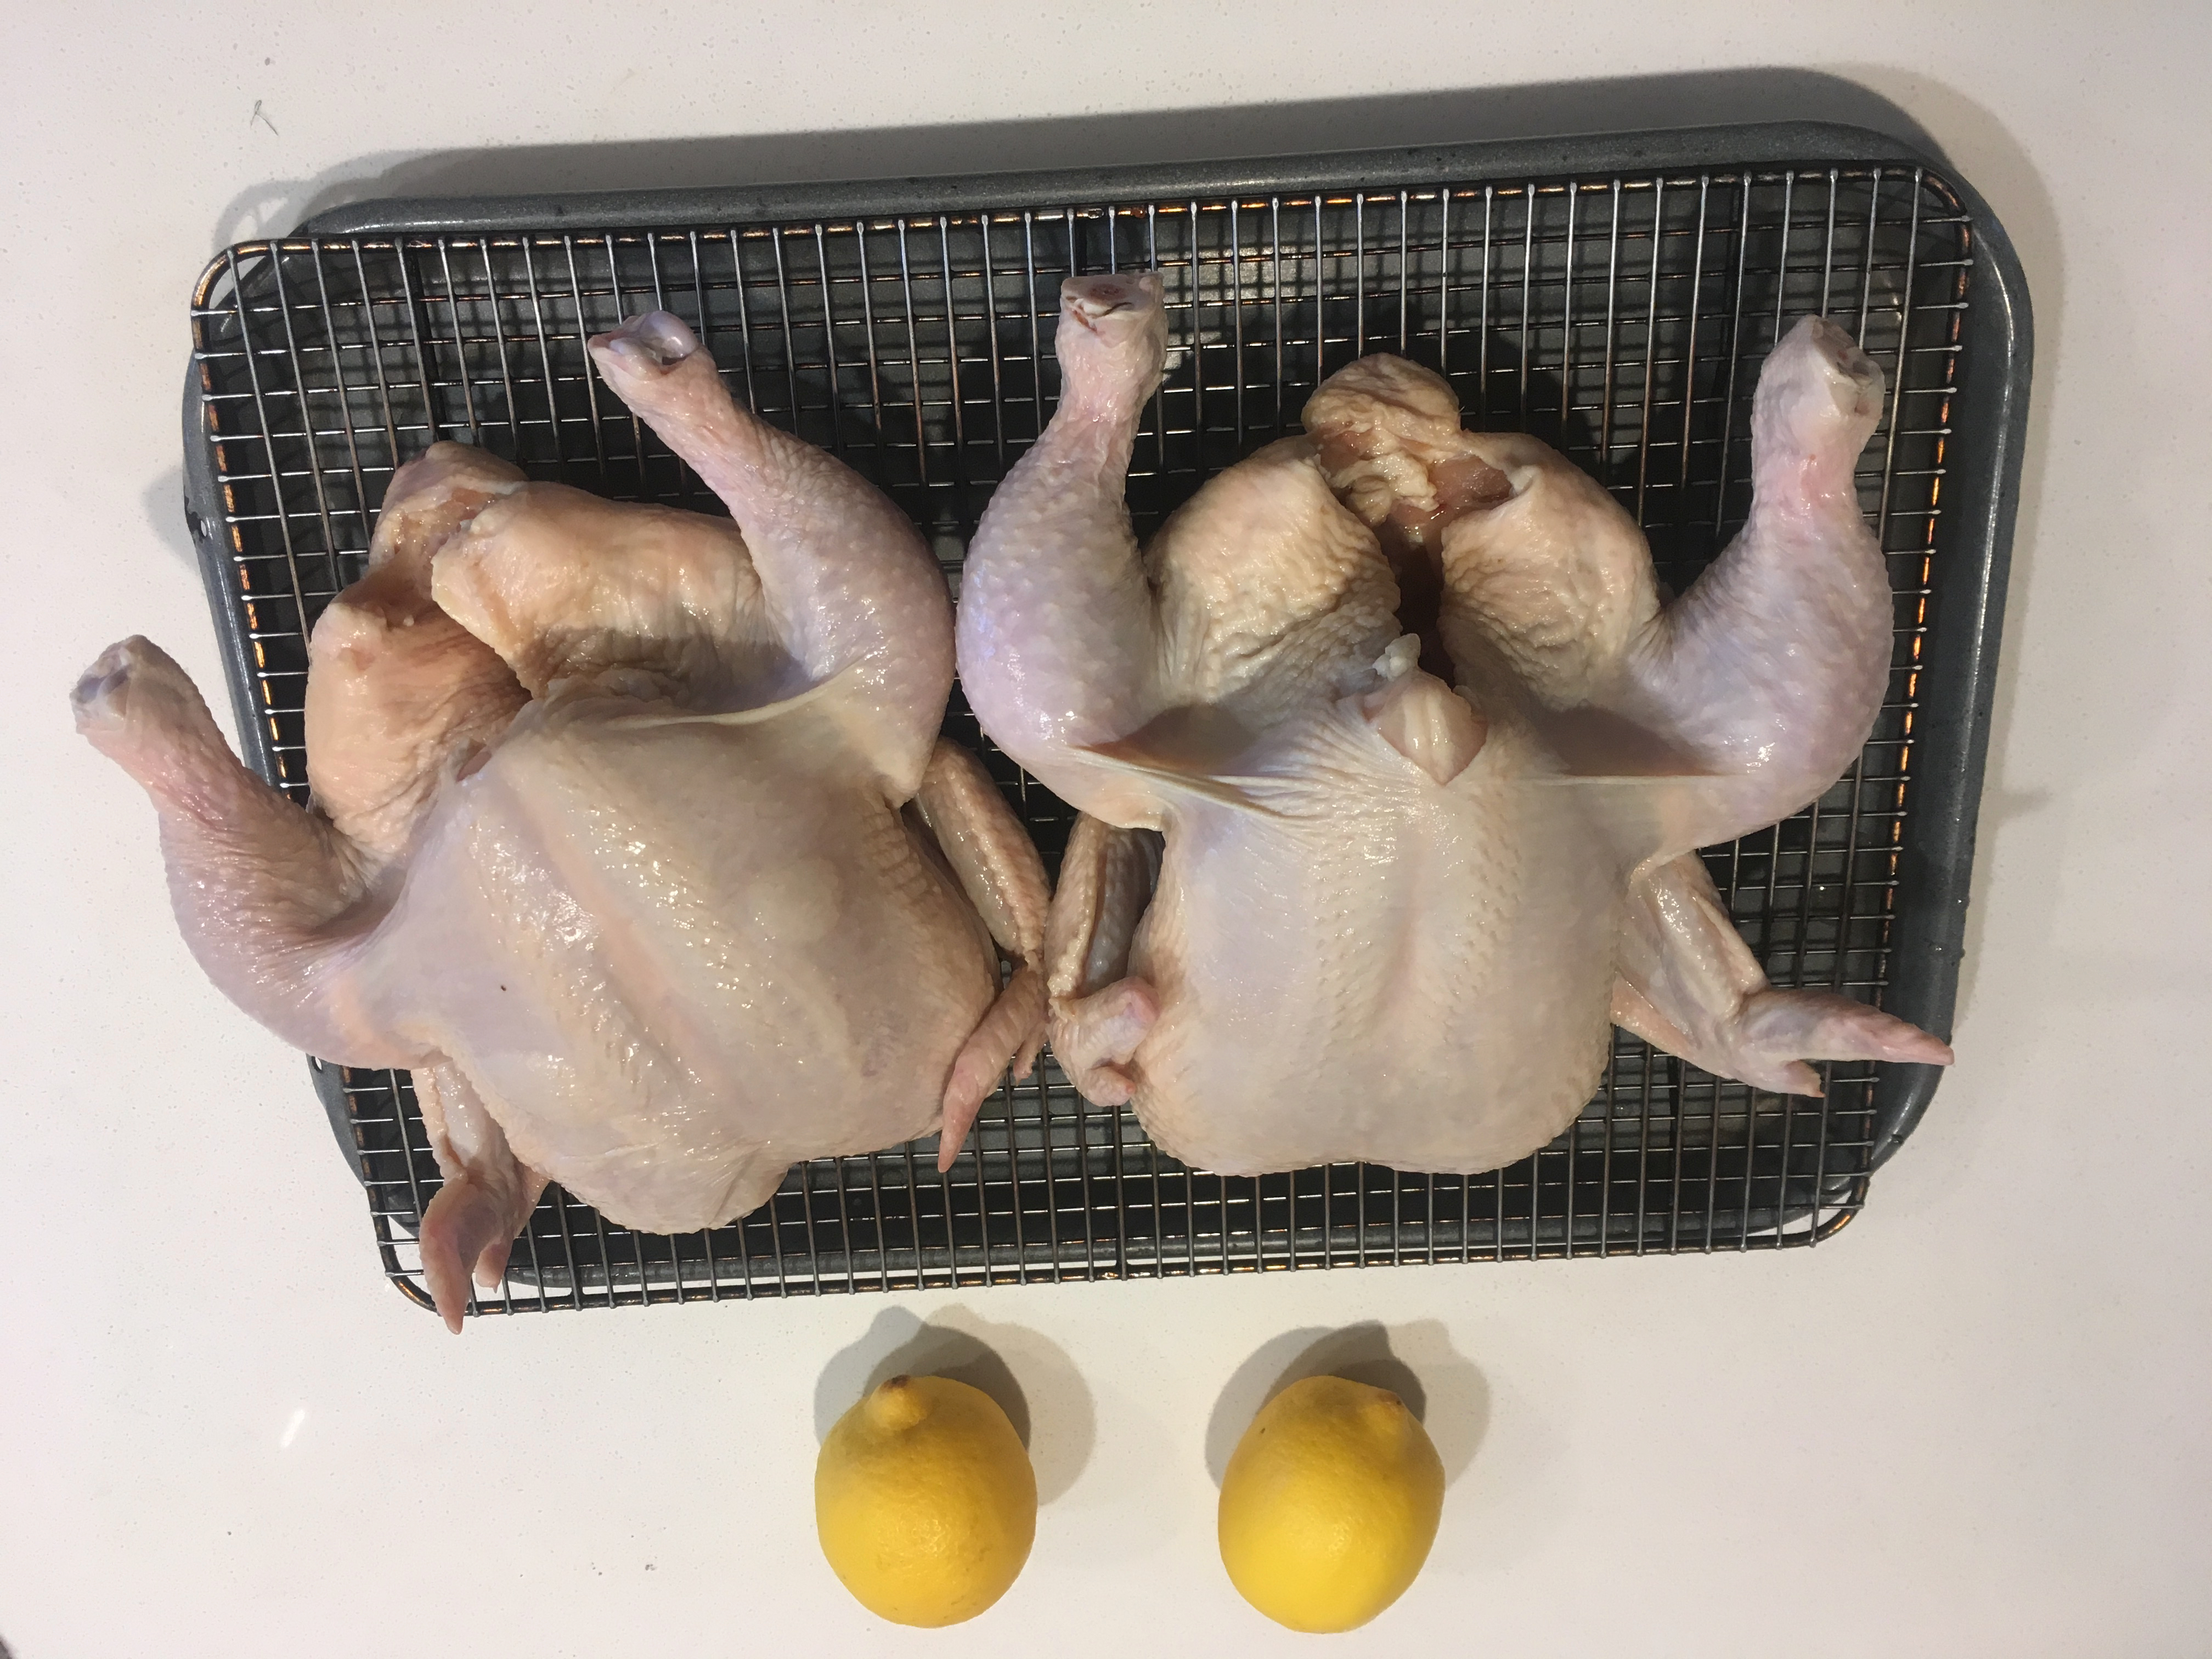
\includegraphics[width=0.25\textwidth]{\imageDir/\fileName/IMG_3197.jpg} &
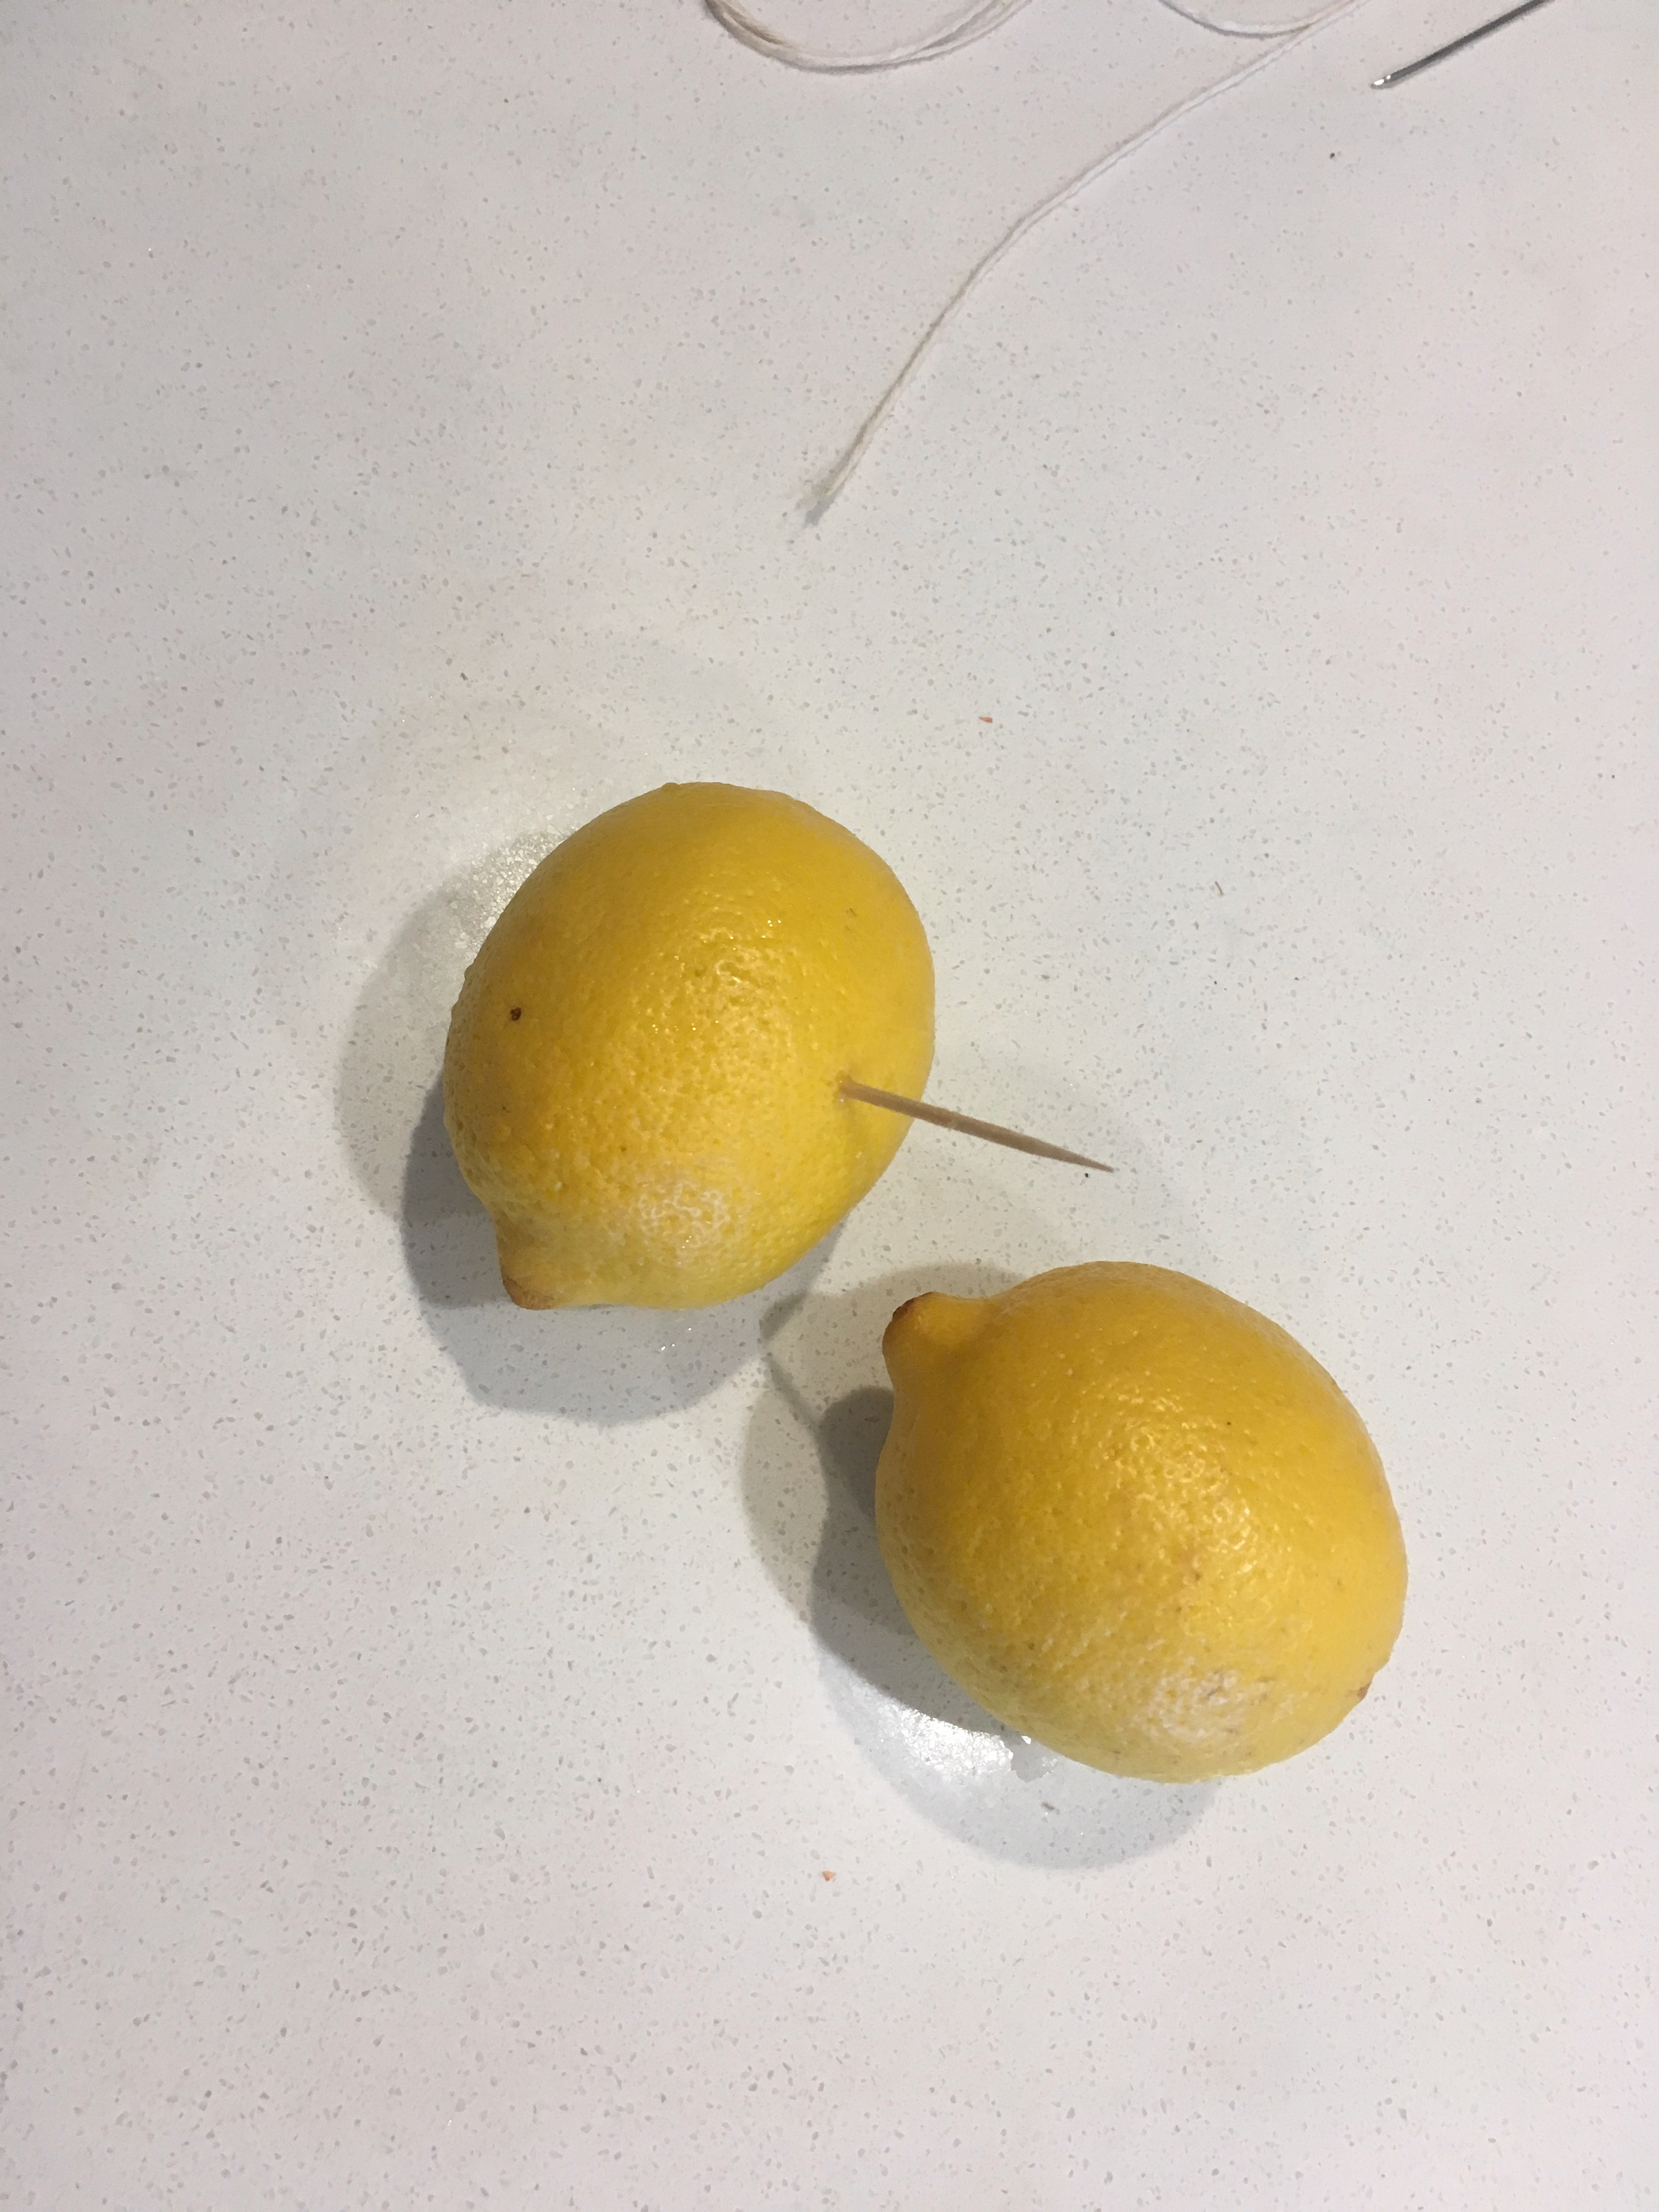
\includegraphics[width=0.25\textwidth]{\imageDir/\fileName/IMG_3212.jpg} &
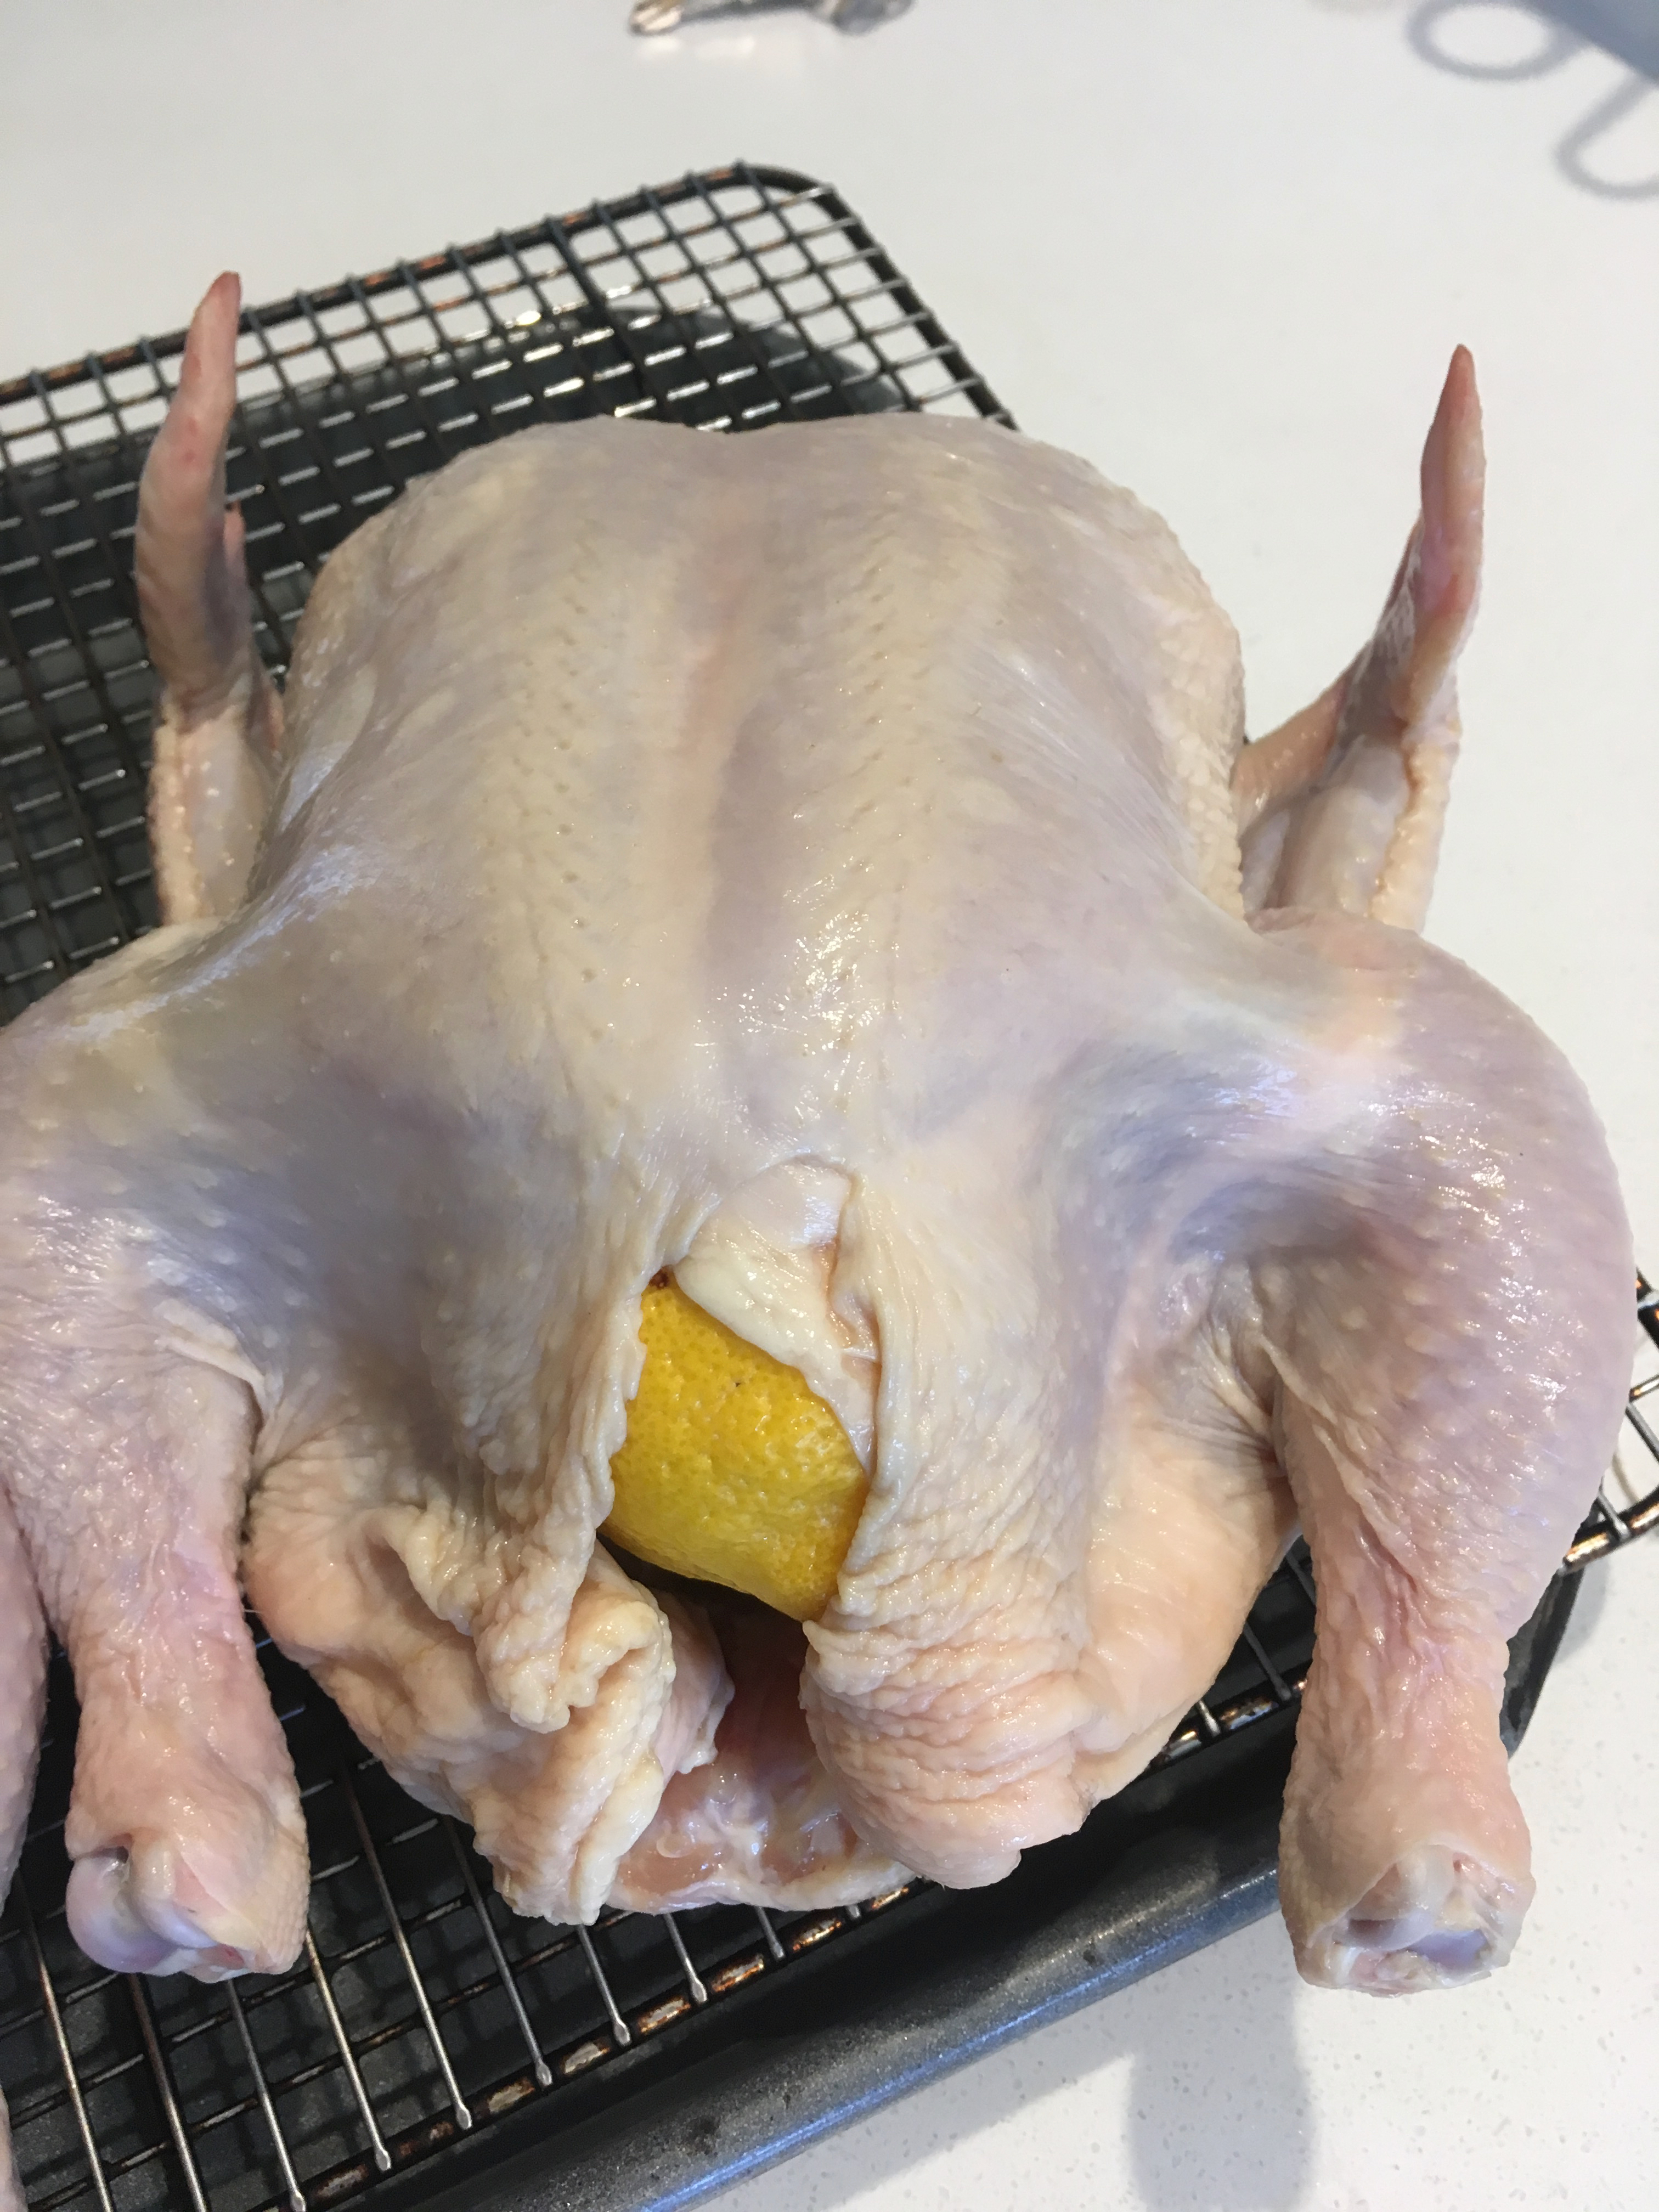
\includegraphics[width=0.25\textwidth]{\imageDir/\fileName/IMG_3213.jpg} \\
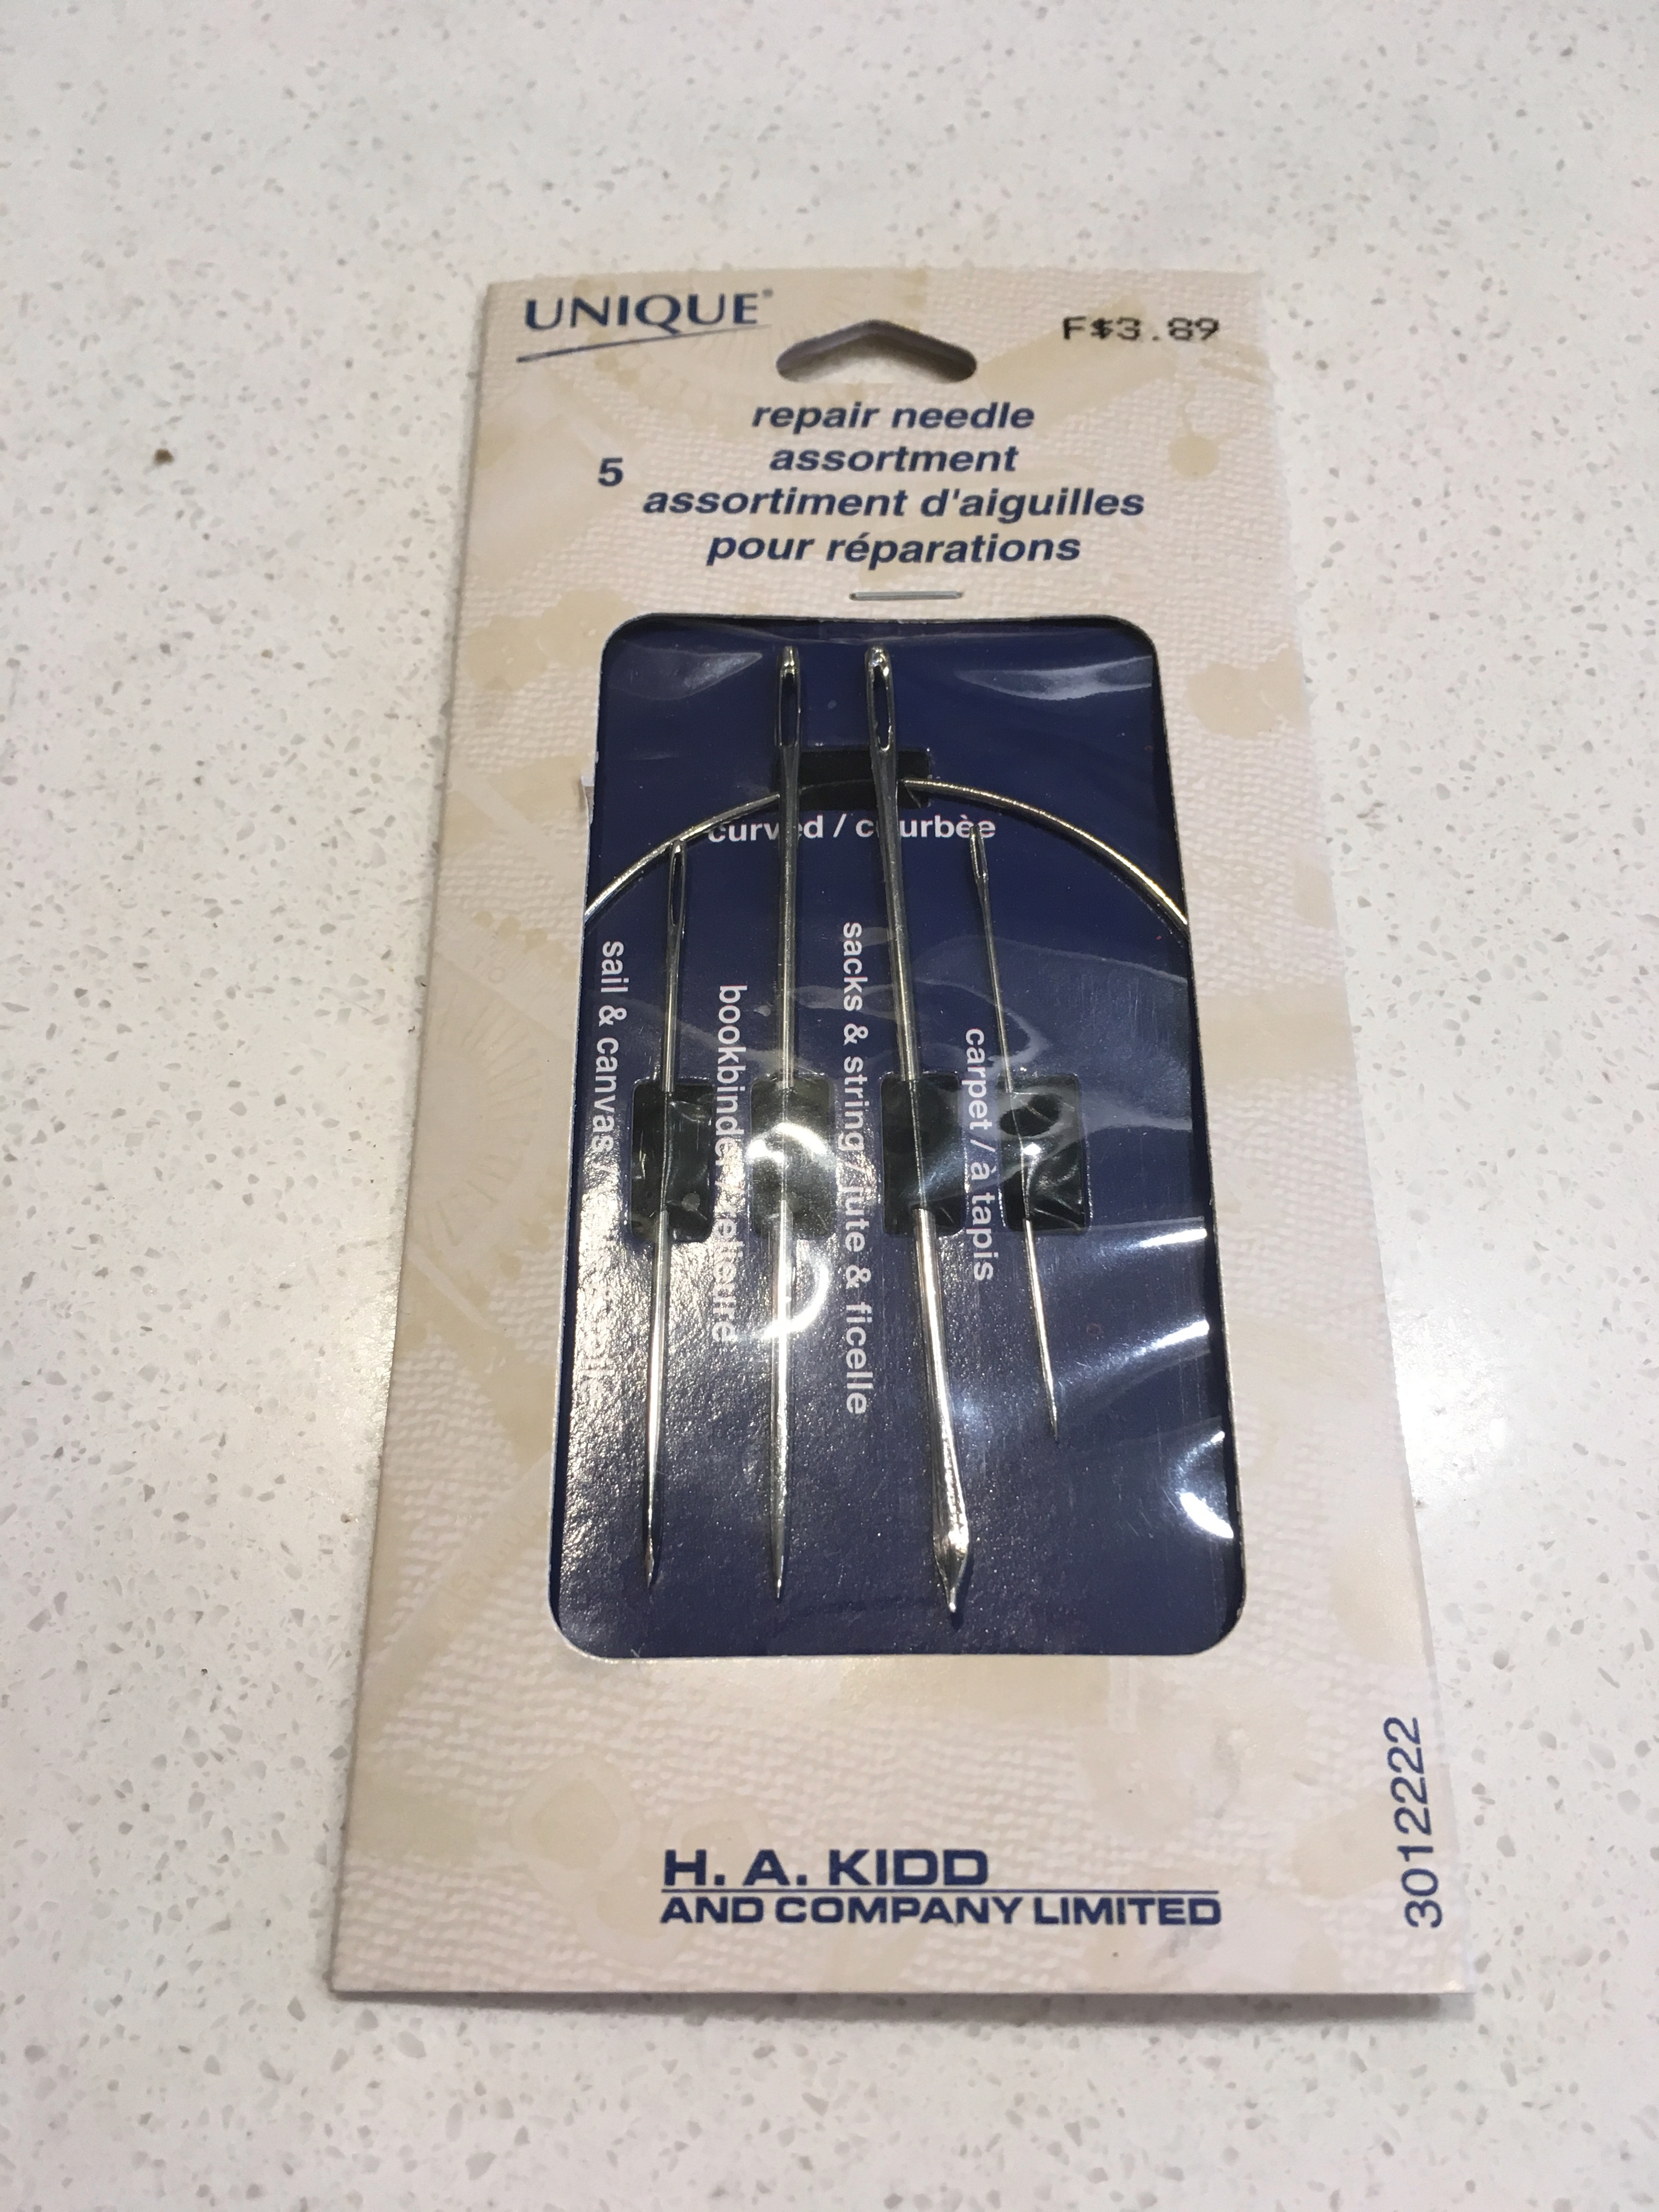
\includegraphics[width=0.25\textwidth]{\imageDir/\fileName/IMG_3206.jpg} &
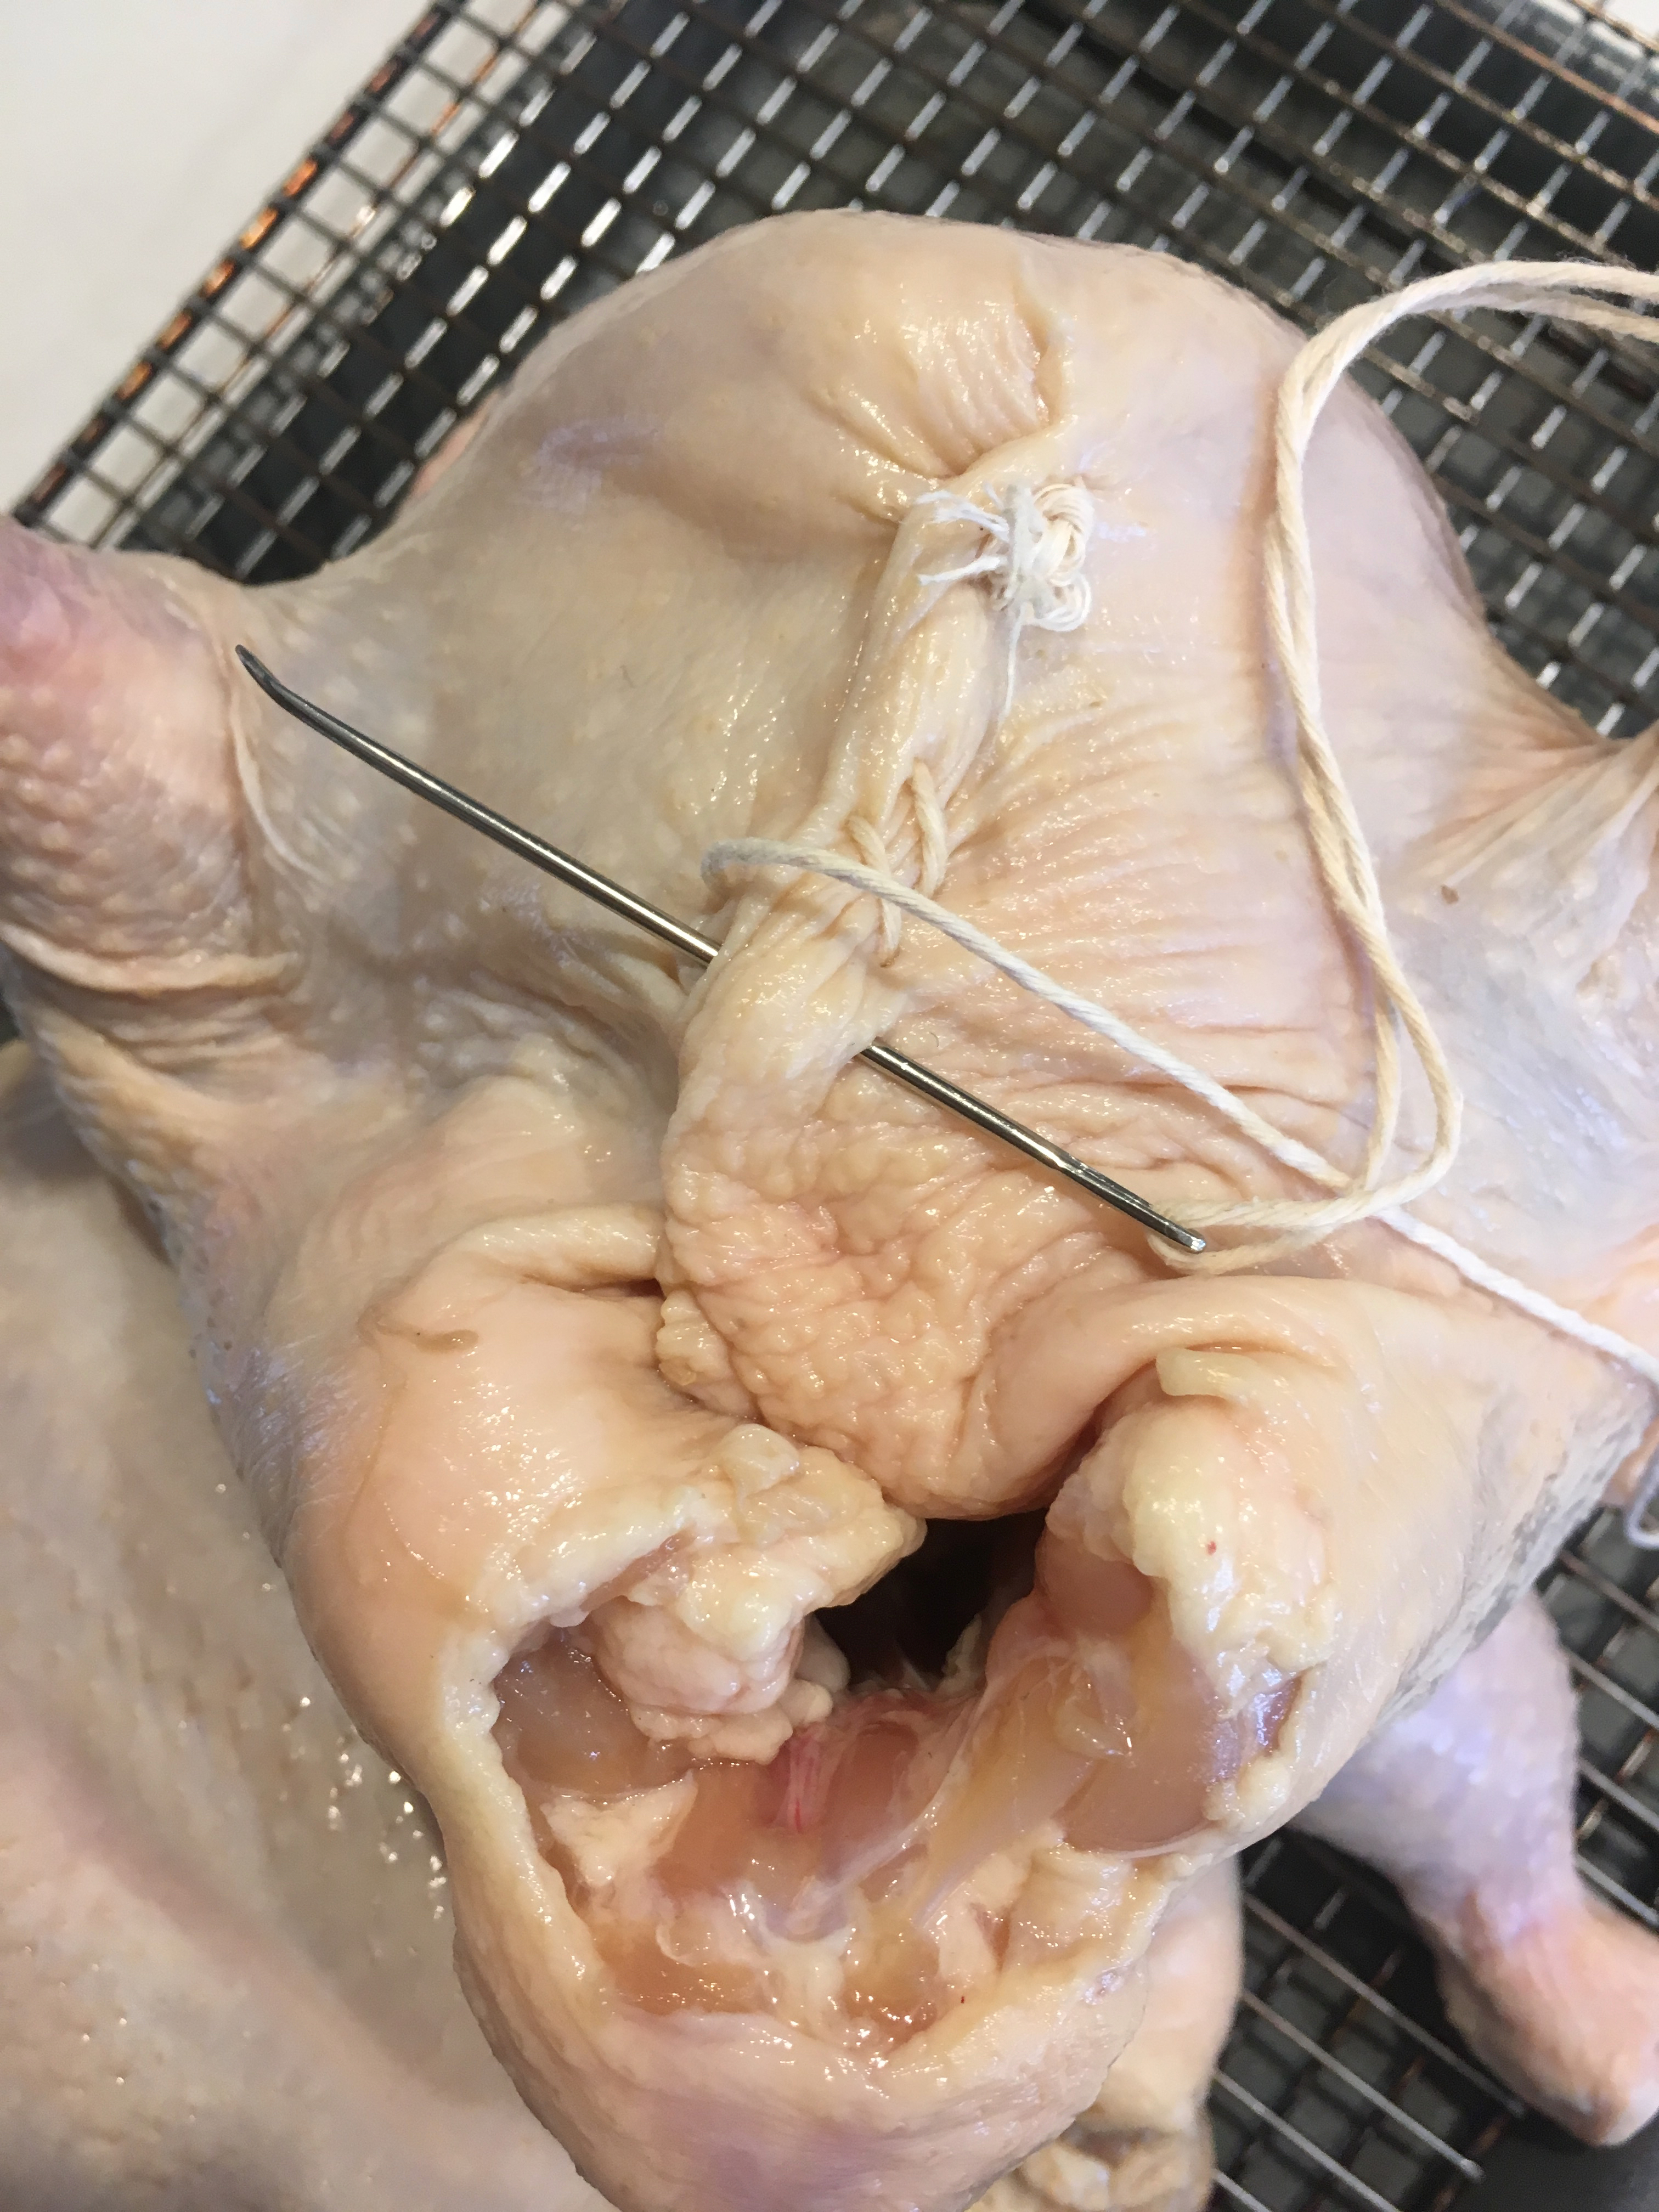
\includegraphics[width=0.25\textwidth]{\imageDir/\fileName/IMG_3214.jpg} &
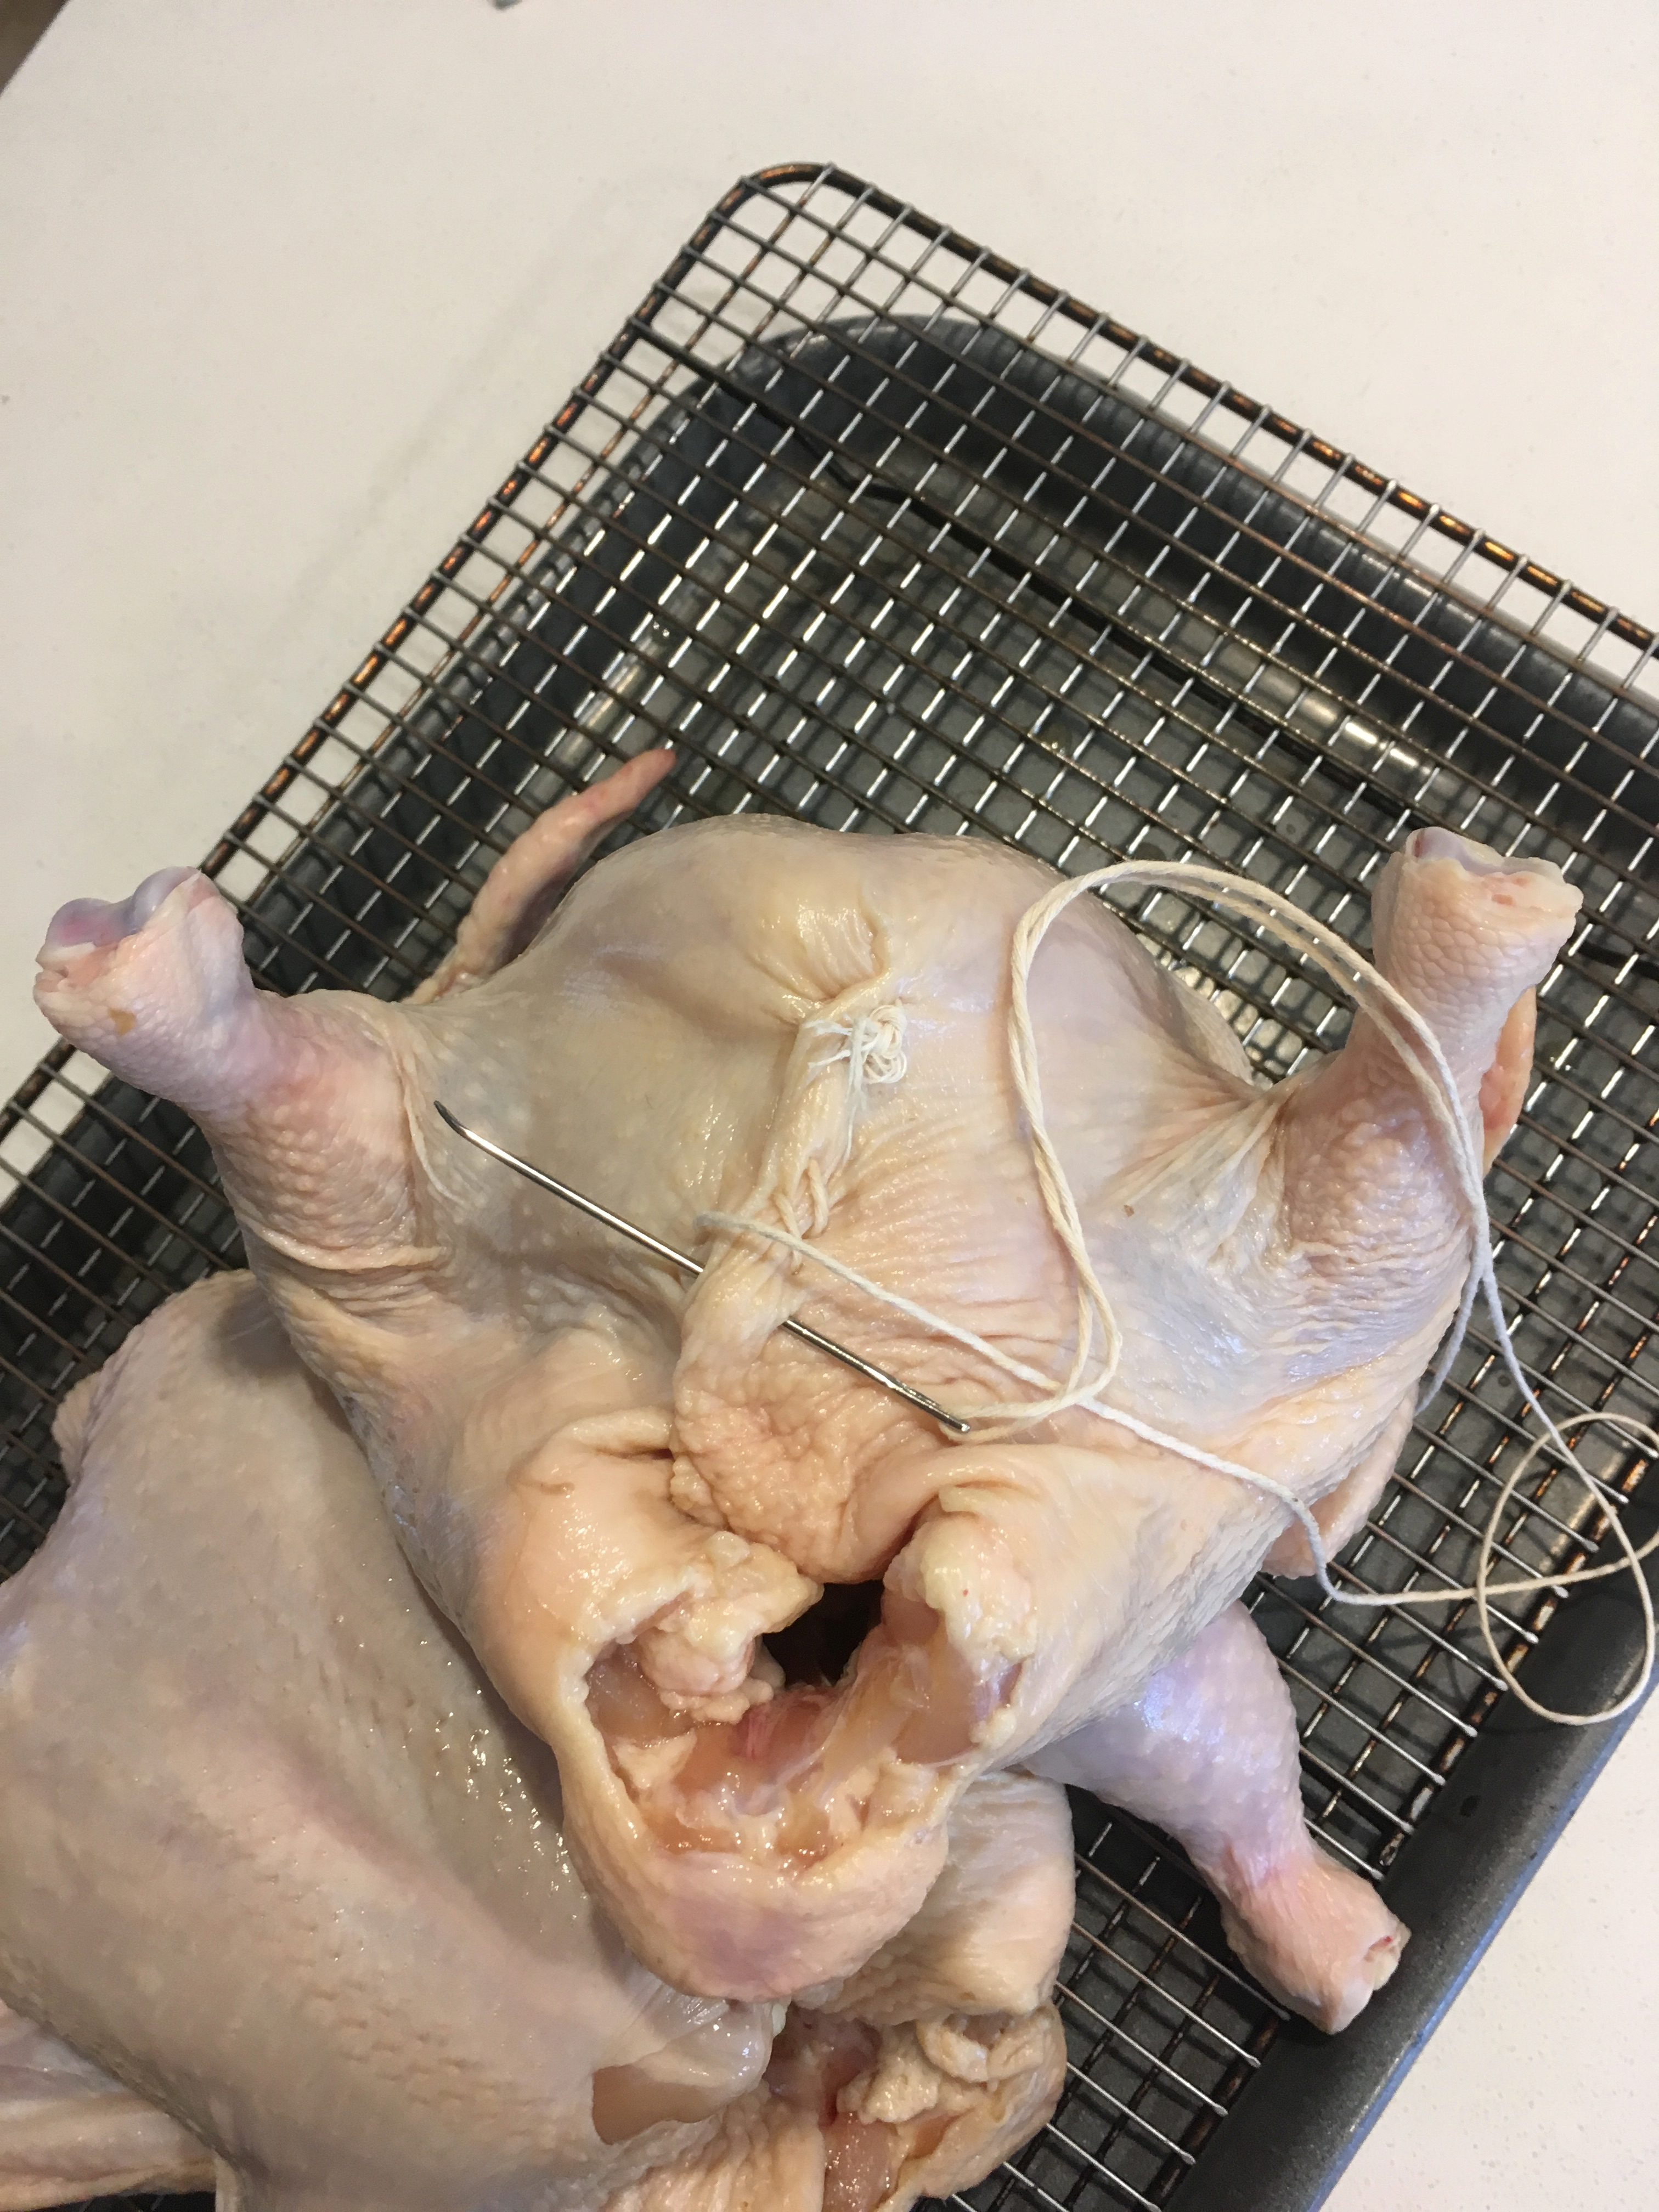
\includegraphics[width=0.25\textwidth]{\imageDir/\fileName/IMG_3216.jpg} \\
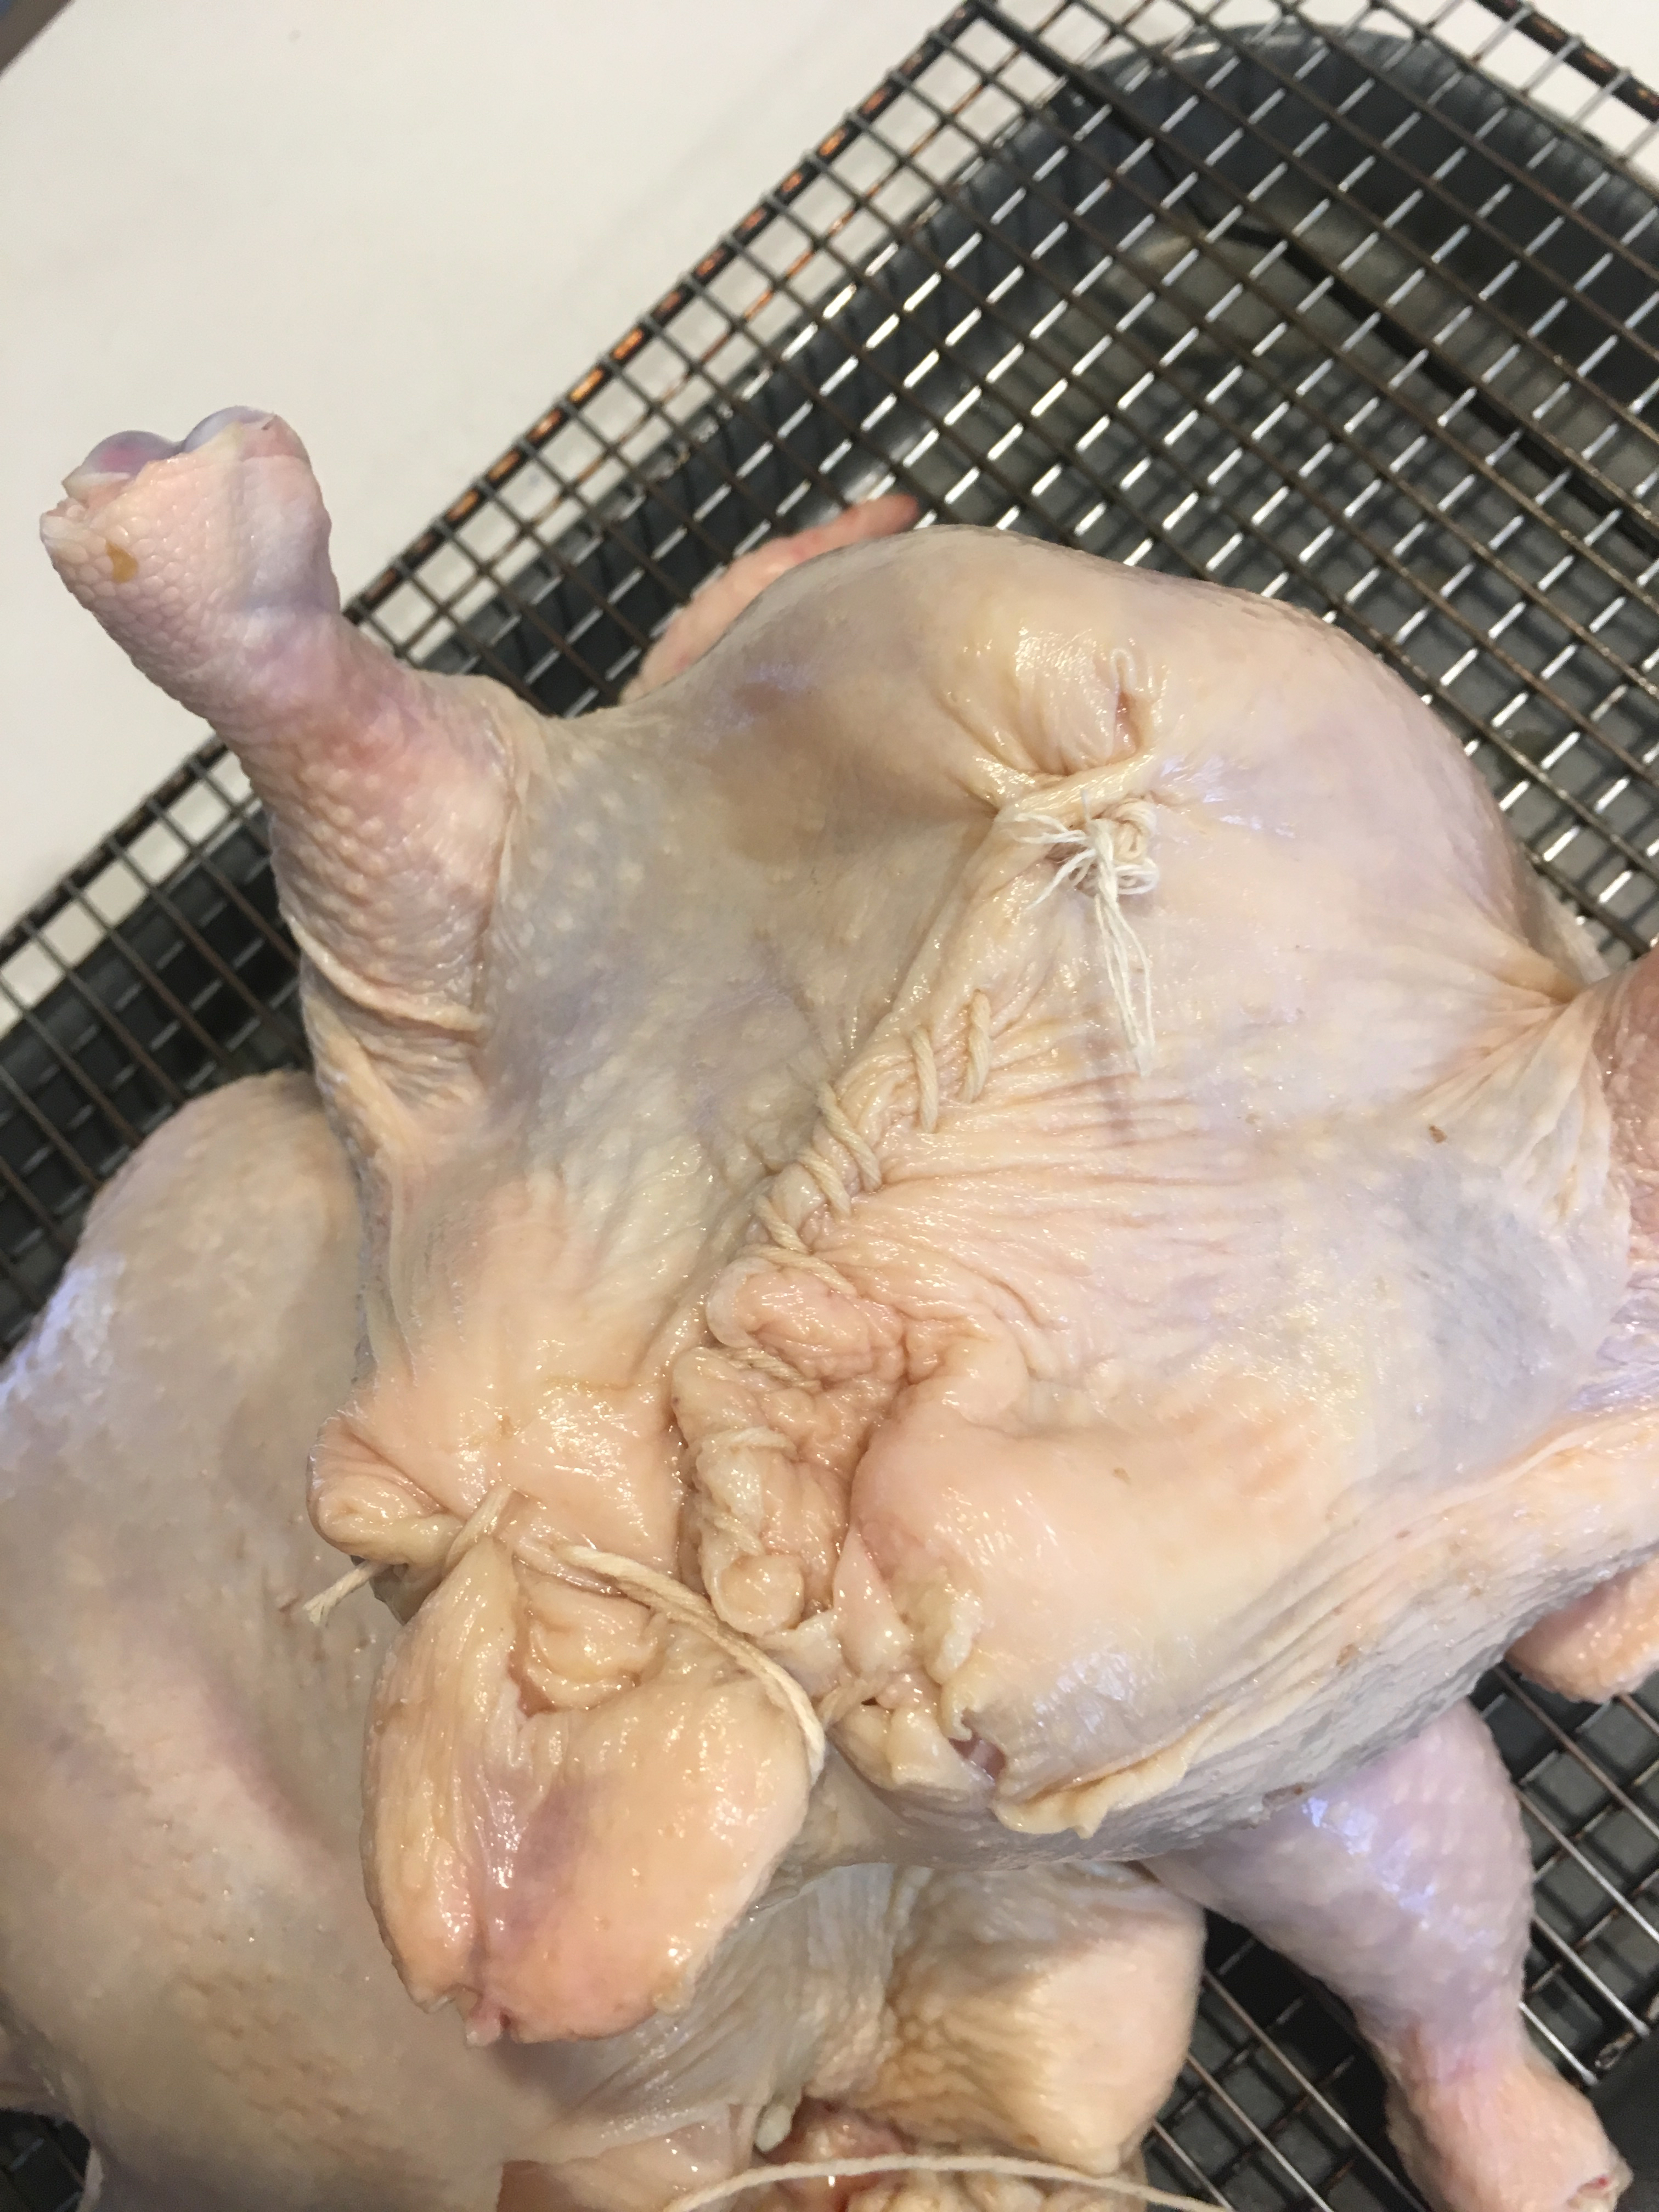
\includegraphics[width=0.25\textwidth]{\imageDir/\fileName/IMG_3217.jpg} &
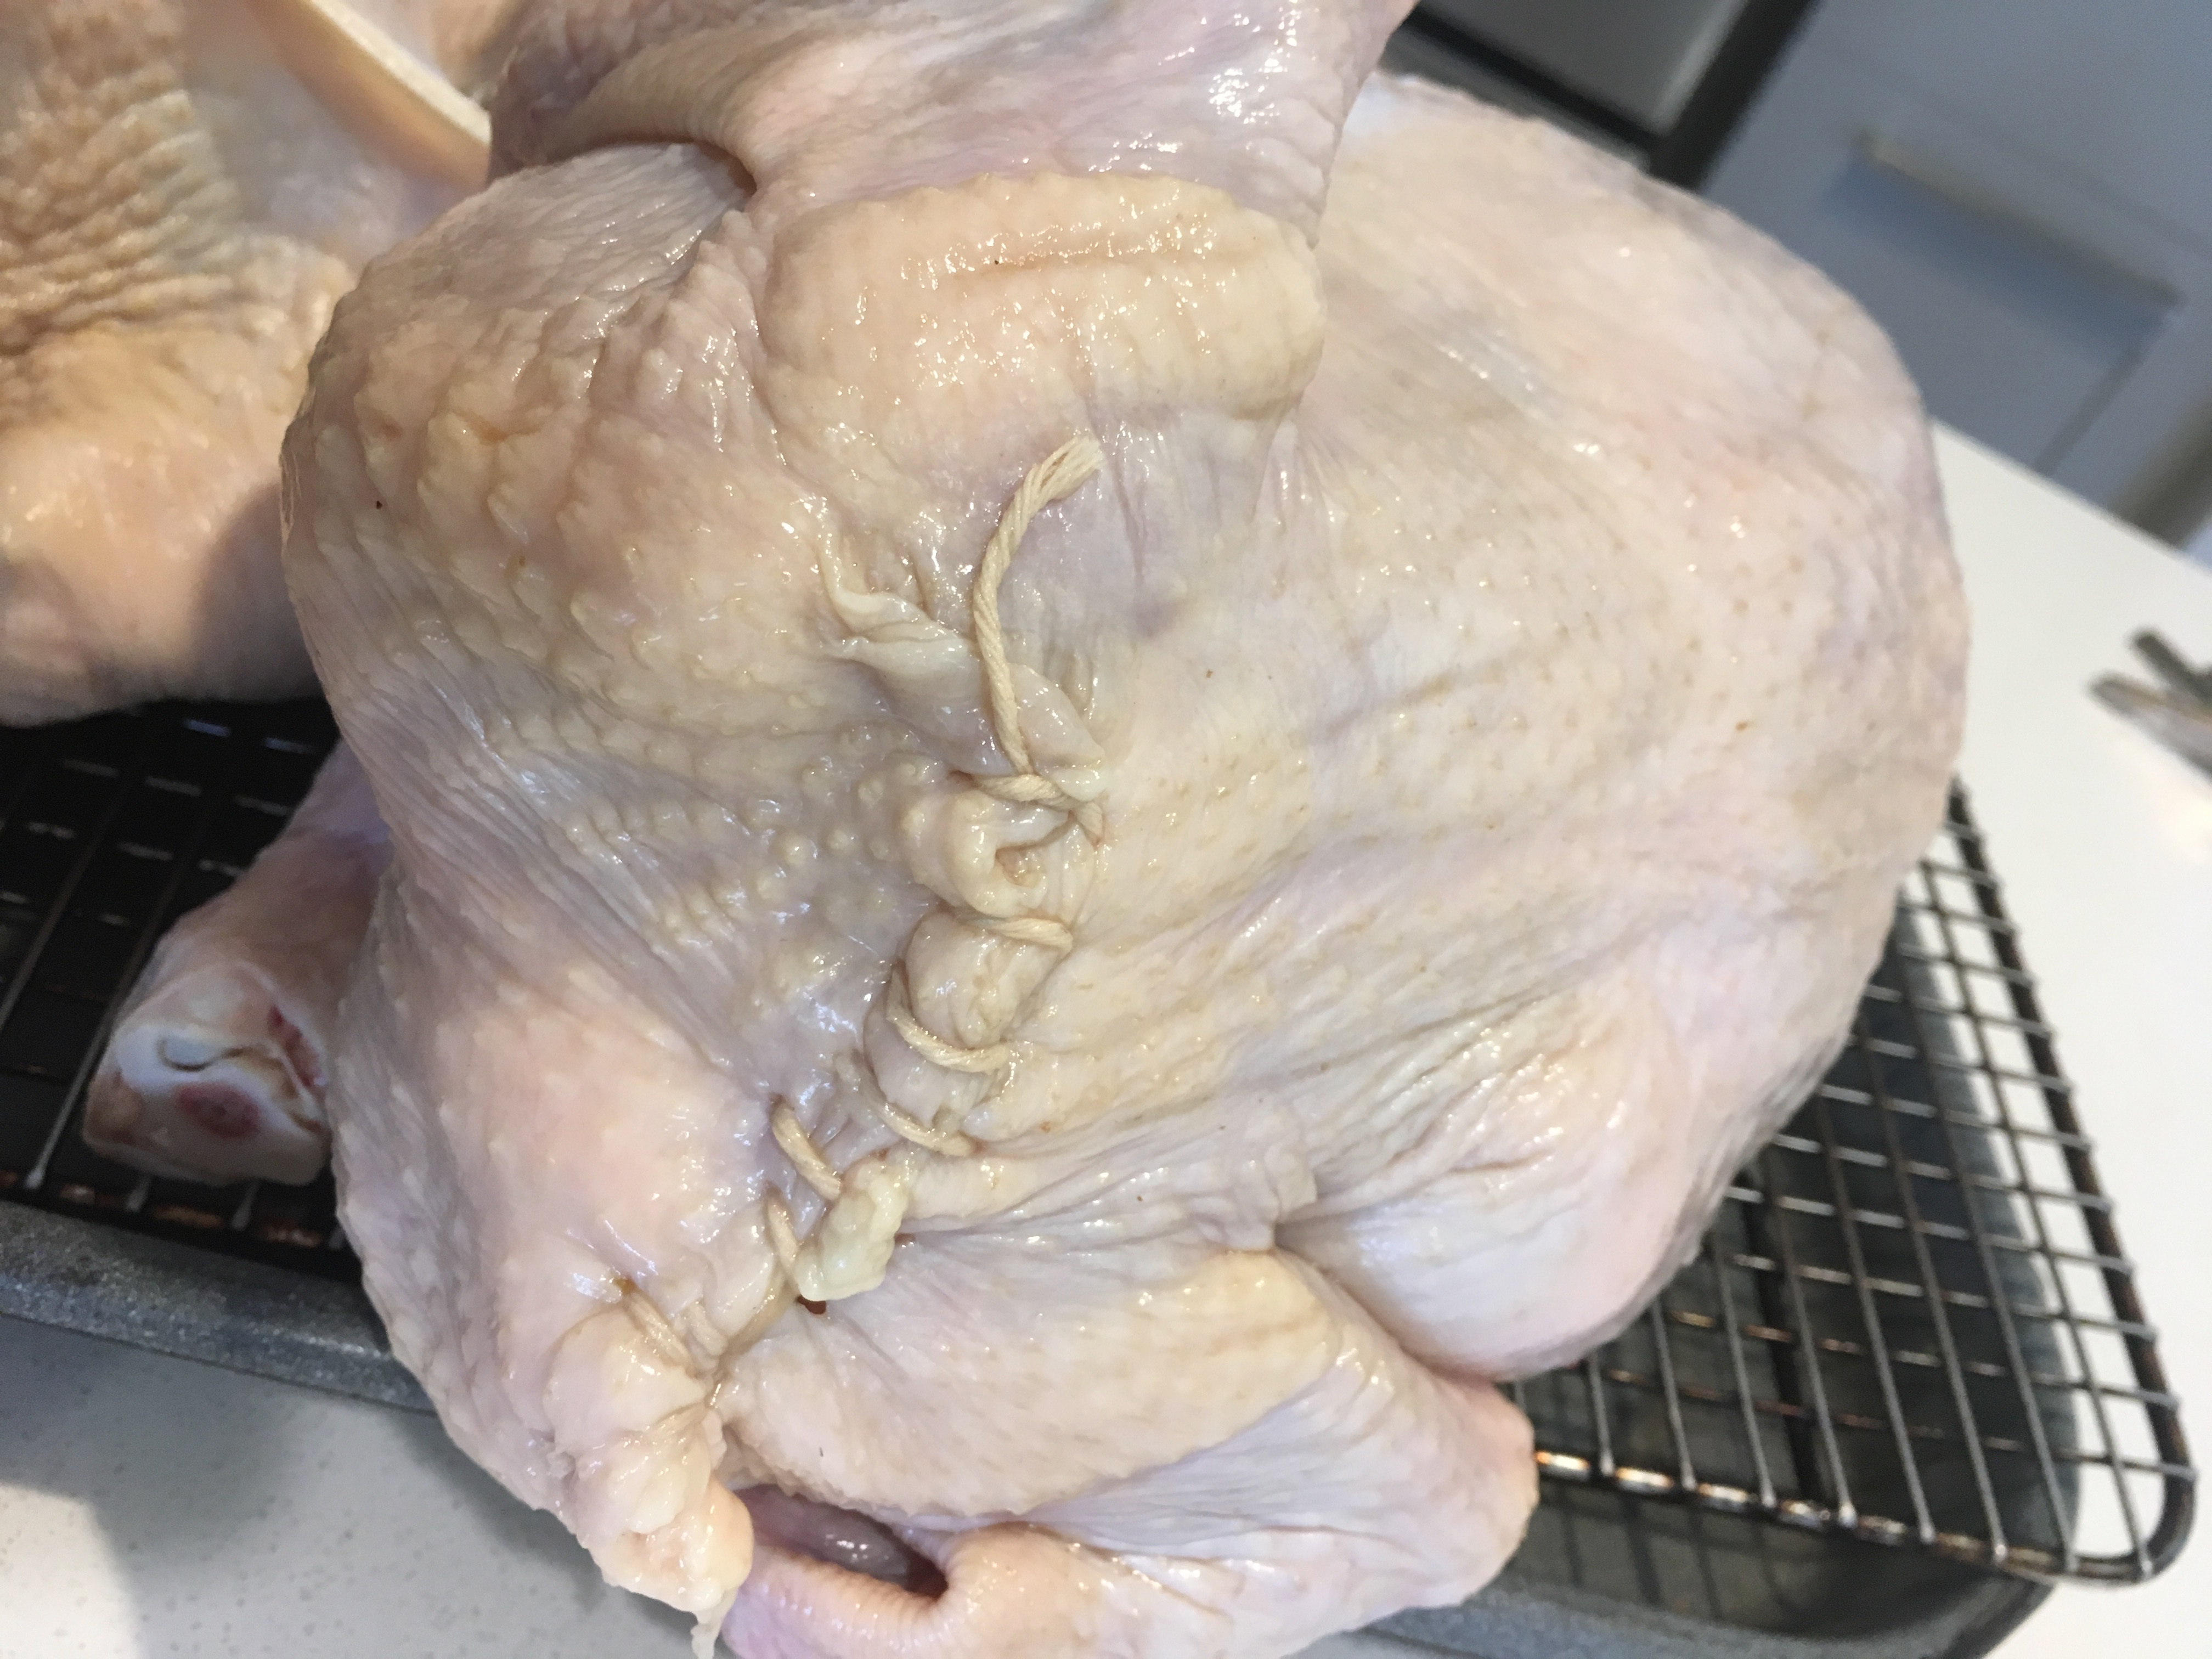
\includegraphics[width=0.25\textwidth]{\imageDir/\fileName/IMG_3218.jpg} &
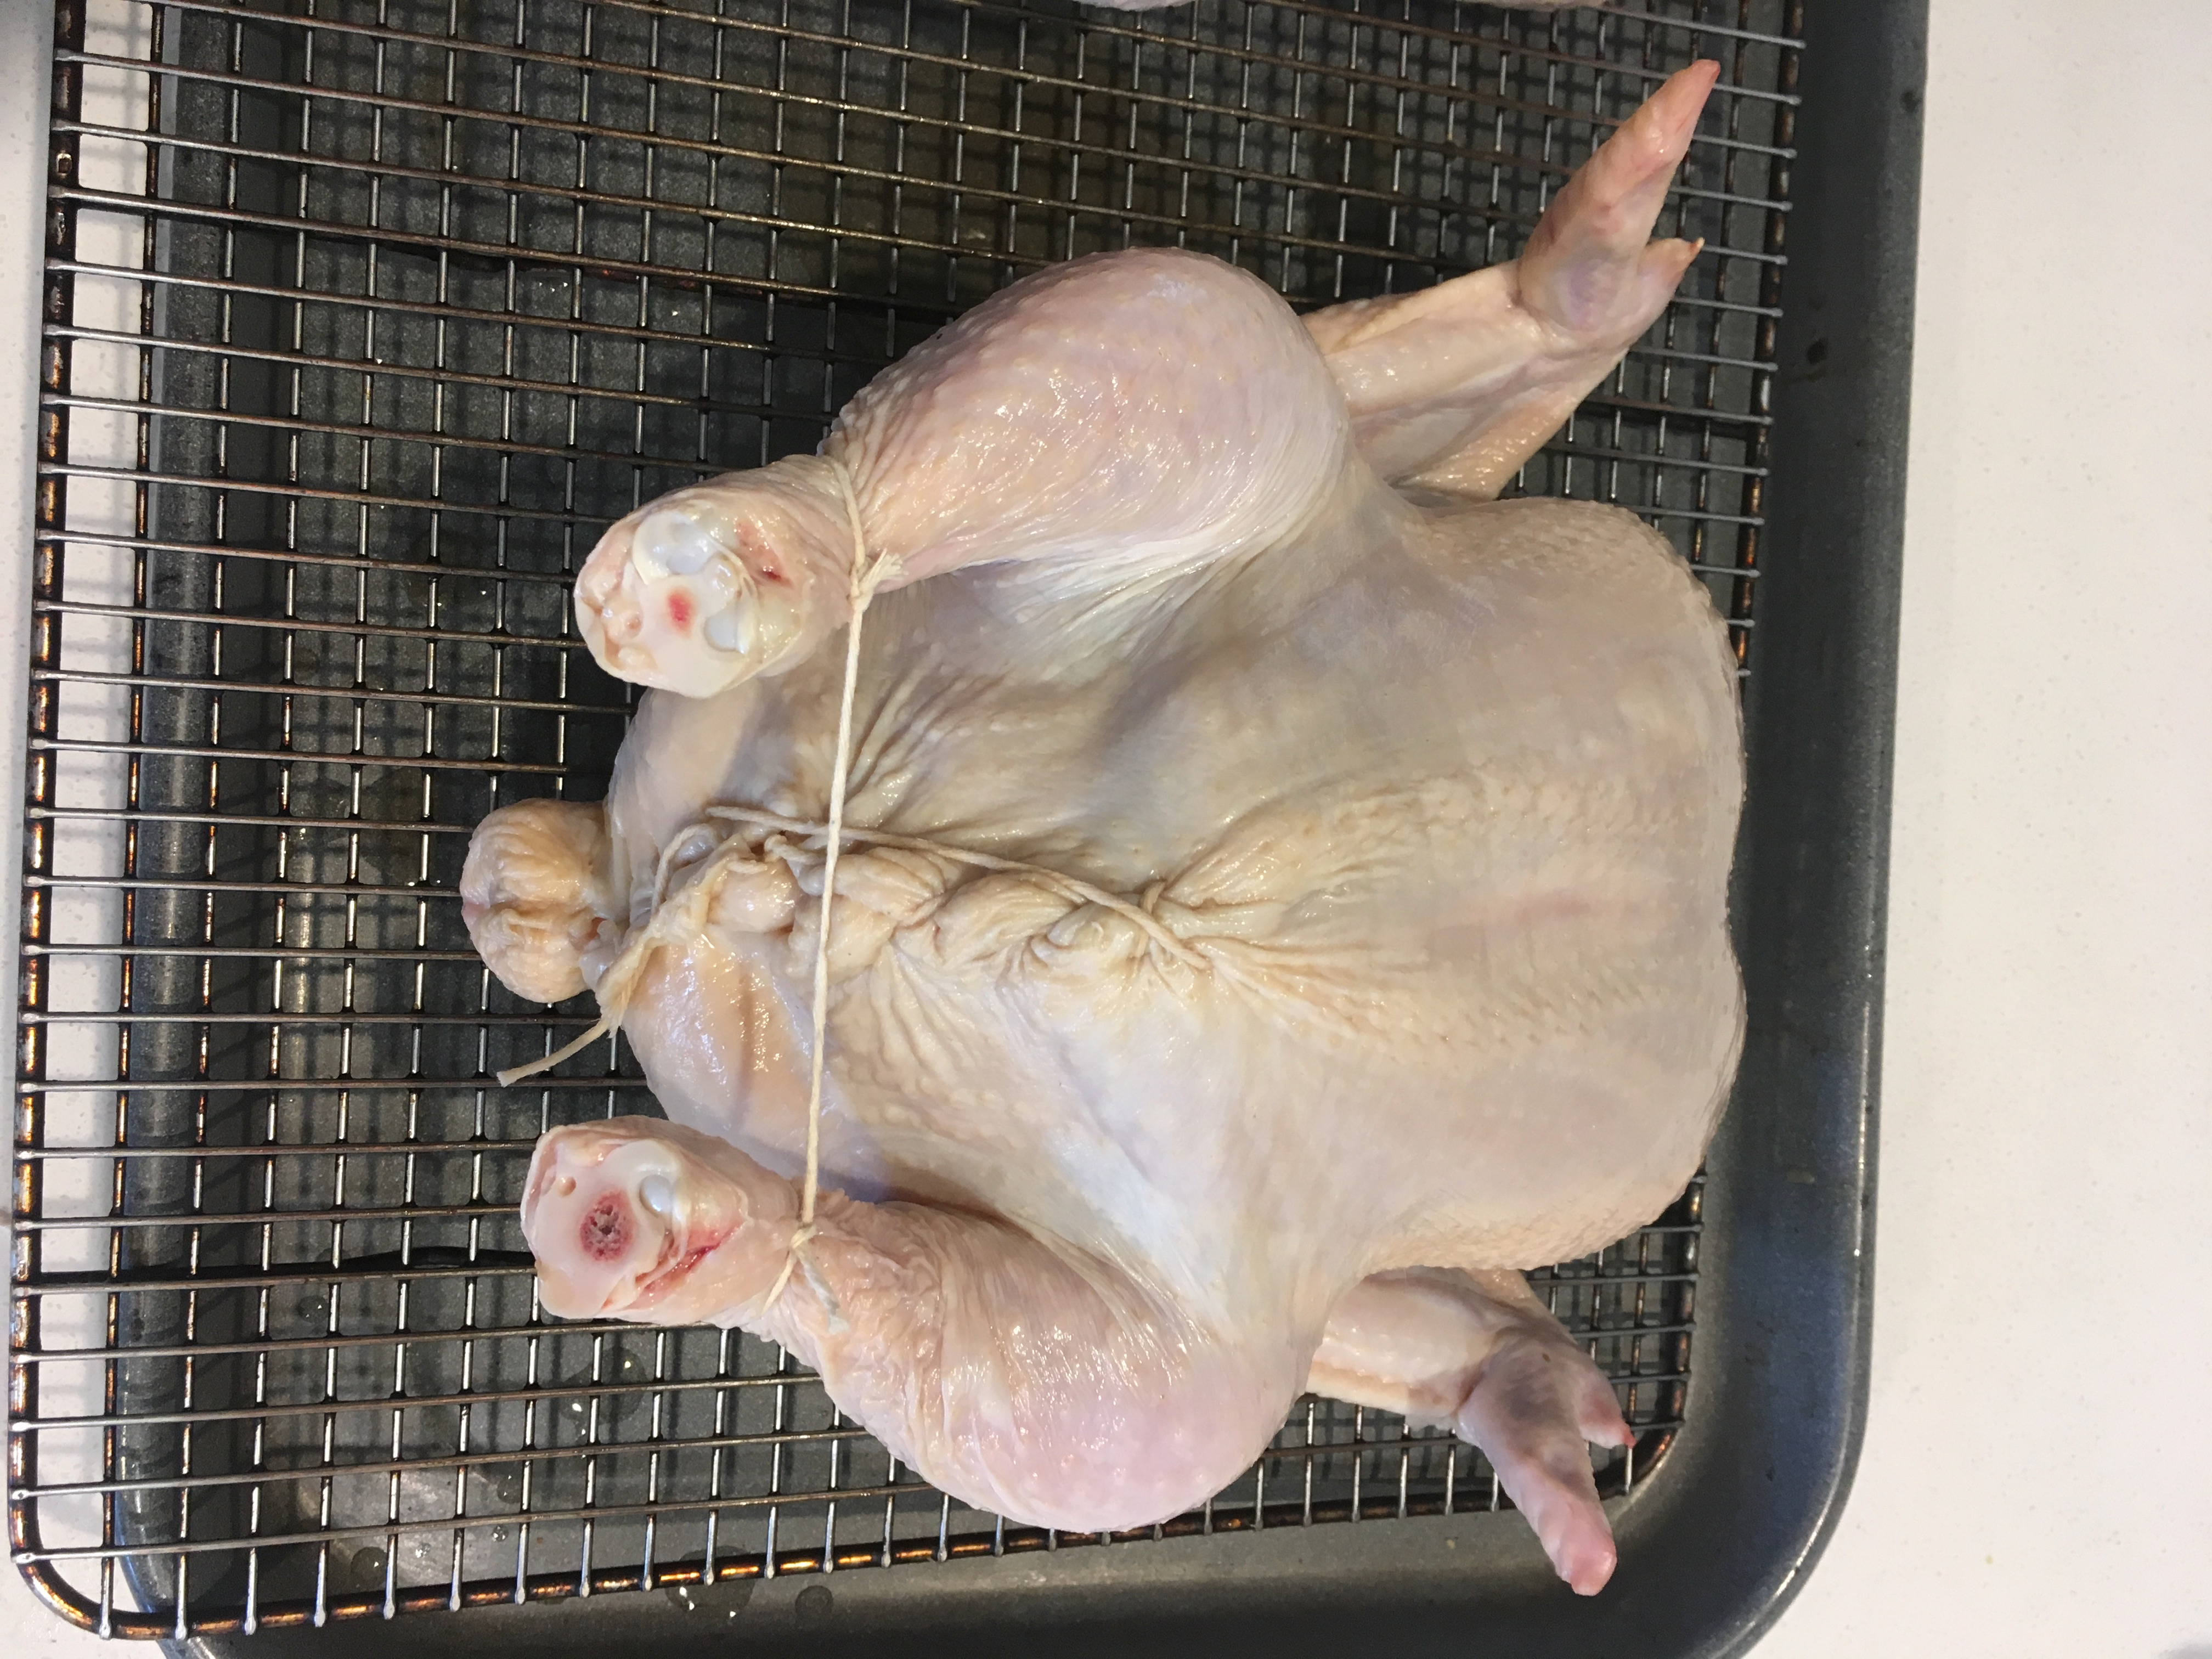
\includegraphics[width=0.25\textwidth]{\imageDir/\fileName/IMG_3219.jpg} \\
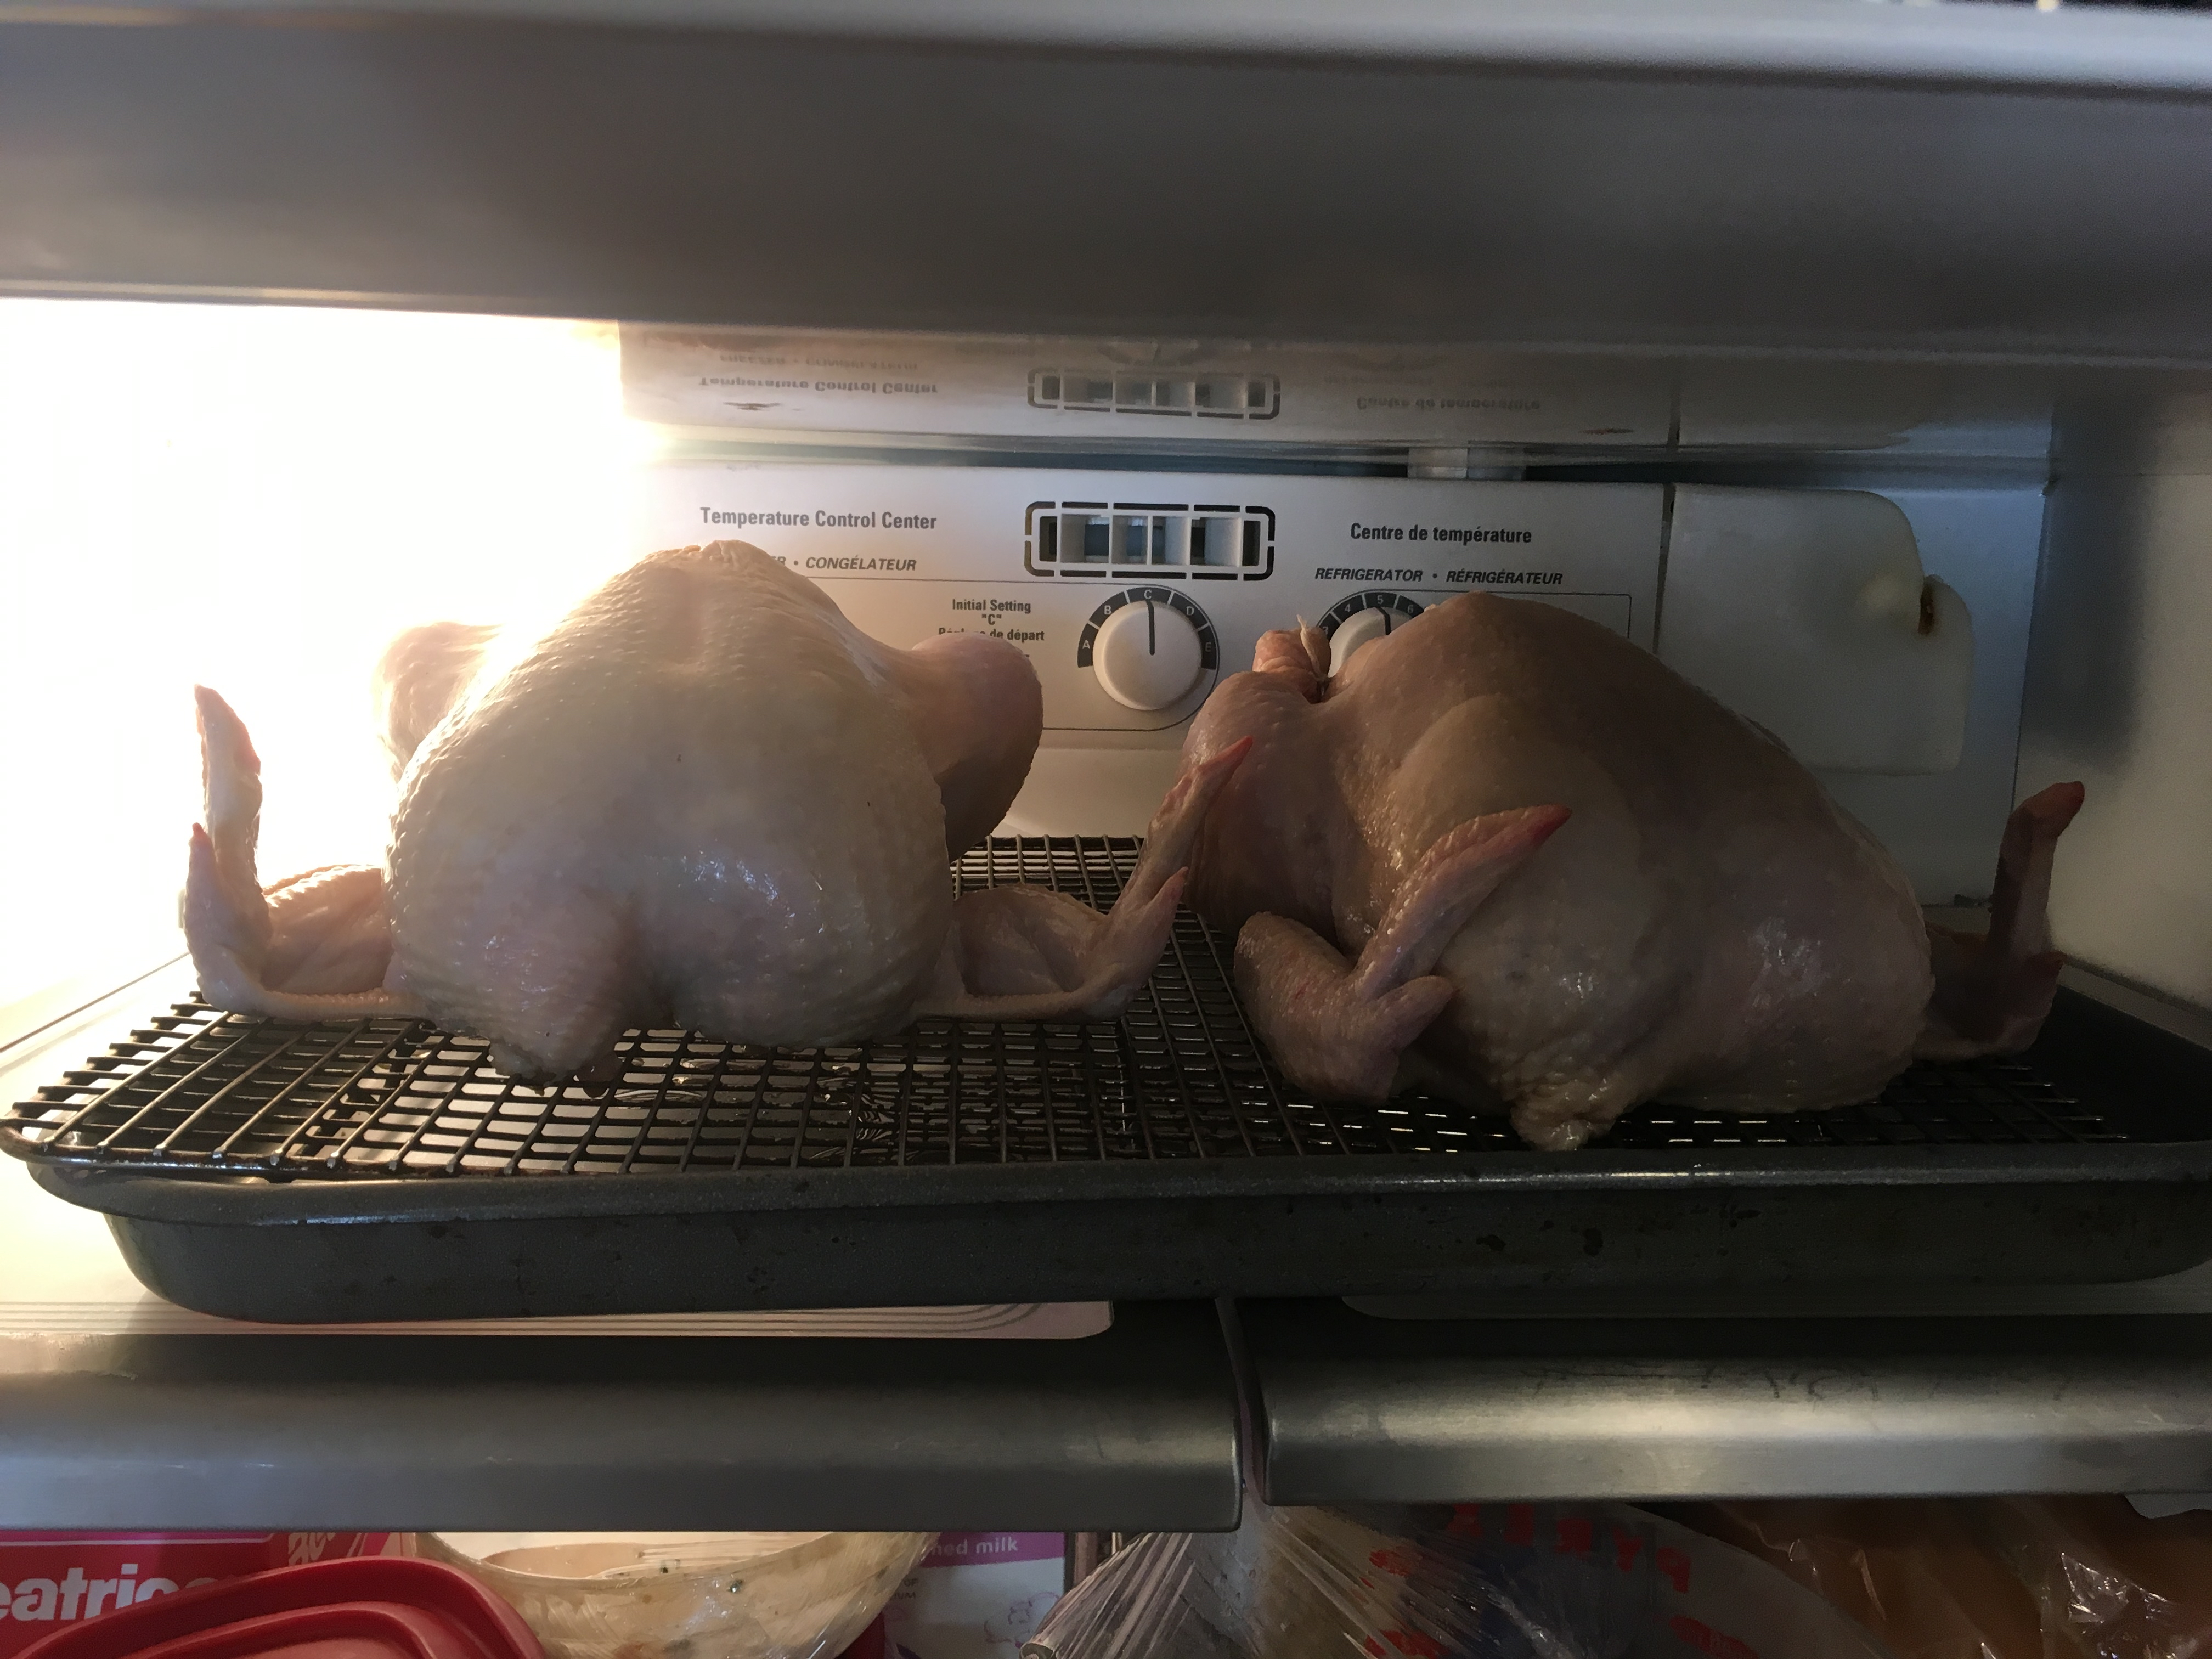
\includegraphics[width=0.25\textwidth]{\imageDir/\fileName/IMG_3220.jpg} &
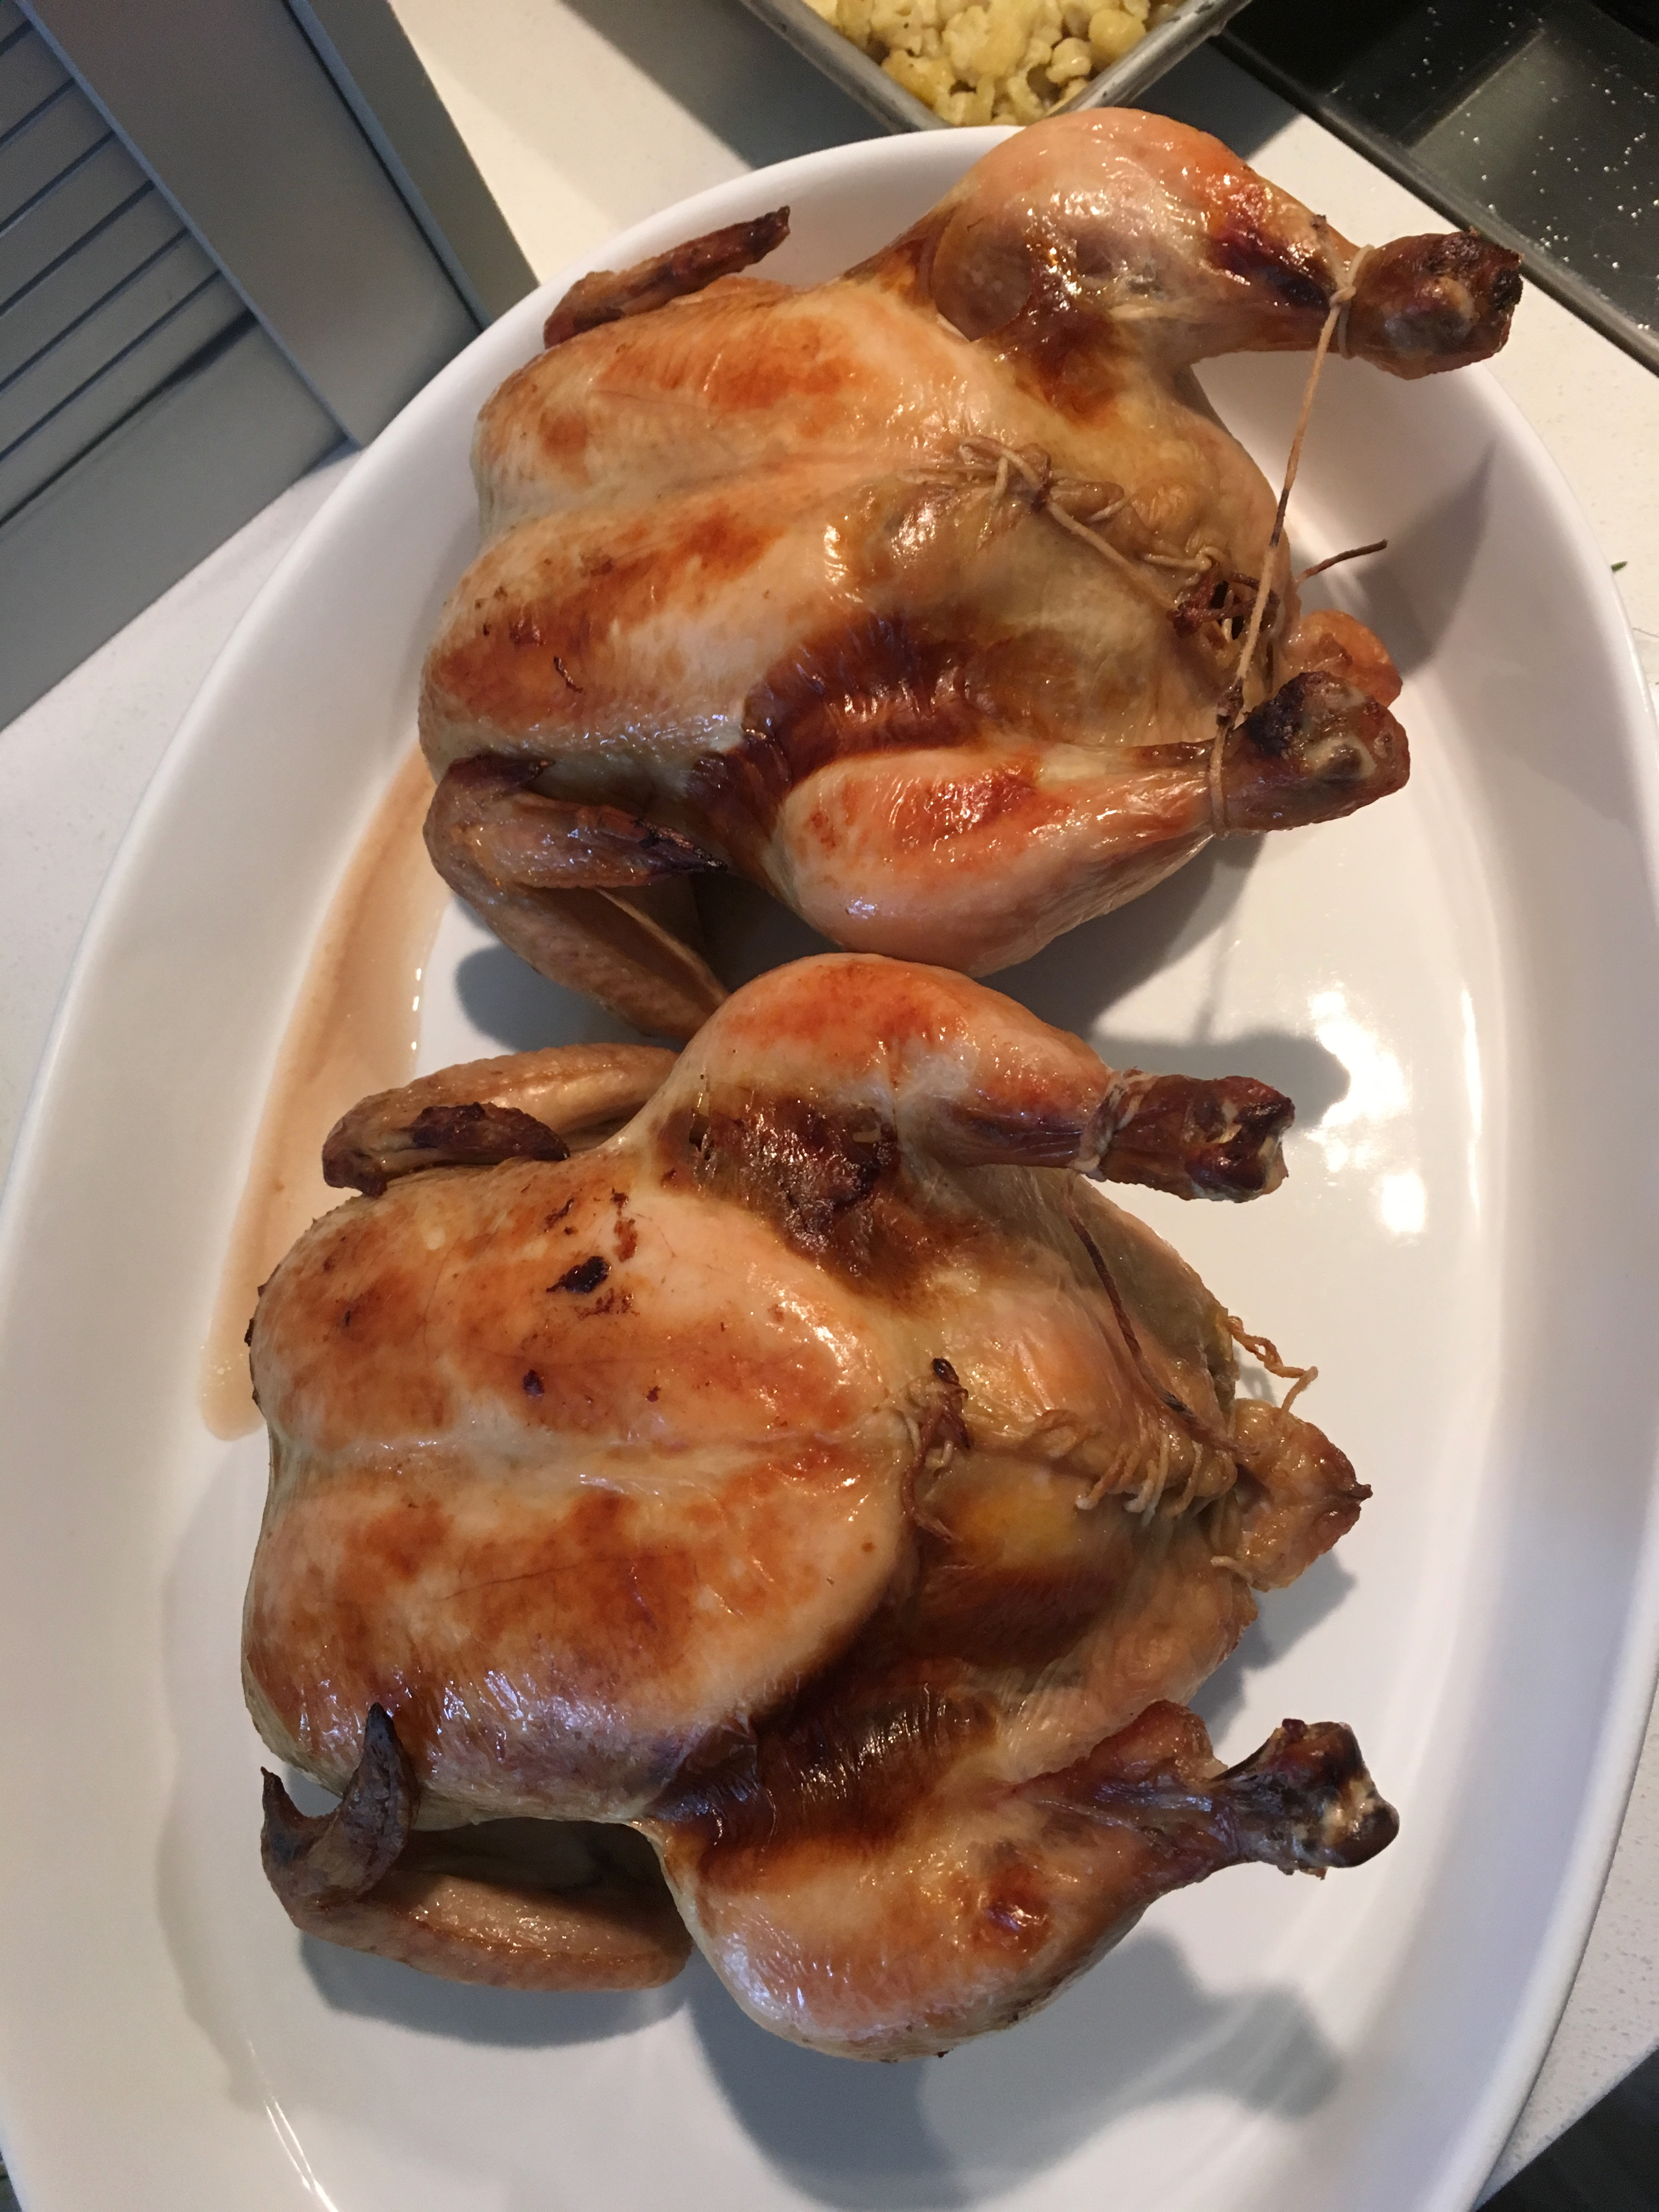
\includegraphics[width=0.25\textwidth]{\imageDir/\fileName/IMG_3228.jpg} \\
\end{tabular}
\end{table}


\end{document}



